\documentclass[a4paper,  11pt]{ctexart}
\usepackage{srcltx,graphicx}
\usepackage{amsmath, amssymb, amsthm}
\usepackage{color}
\usepackage{lscape}
\usepackage{multirow}
\usepackage{psfrag}
\usepackage{diagbox}
\usepackage[hang]{subfigure}
\usepackage{float}
\usepackage[colorlinks,linkcolor=black,anchorcolor=blue,citecolor=green]{hyperref}

\newtheorem{theorem}{Theorem}
\newtheorem{lemma}{Lemma}
\newtheorem{definition}{Definition}
\newtheorem{comment}{Comment}
\newtheorem{conjecture}{Conjecture}

\newcommand\bbR{\mathbb{R}}
\newcommand\bbN{\mathbb{N}}
\newcommand\bbC{\mathbb{C}}
\newcommand\bx{\boldsymbol{x}}
\newcommand\dd{\,\mathrm{d}}

\newcommand\diag{\mathrm{diag}}
\newcommand\tr{\mthrm{tr}}

\setlength{\oddsidemargin}{0cm}
\setlength{\evensidemargin}{0cm}
\setlength{\textwidth}{150mm}
\setlength{\textheight}{230mm}

\newcommand\note[2]{{{\bf #1}\color{red} [ {\it #2} ]}}
%\newcommand\note[2]{{ #1 }} % using this line in the formal version

\newcommand\pd[2]{\dfrac{\partial {#1}}{\partial {#2}}}
\newcommand\od[2]{\dfrac{\dd {#1}}{\dd {#2}}}
\newcommand{\bm}[1]{\mbox{\boldmath{$#1$}}}

\begin{document}
\title{差分方法上机作业}
\author{郑灵超\\
160110040
}  
\maketitle
% \tableofcontents
% \newpage
\section{Burgers方程}
\subsection{问题描述}
Burgers方程是经典的偏微分方程,其守恒形式为
\begin{equation}
  \label{eq:Burgers}
  \pd{u}{t}+\pd{(\frac 12u^2)}{x}=0
\end{equation}
我们这里初始值设为分片常数,
\begin{align}
  u_0(x)=\left\{
  \begin{aligned}
    &u_l \quad & x \leq x_1 \\
    &u_m \quad & x_1<x\leq x_2 \\
    &u_r \quad & x > x_2
  \end{aligned}
  \right.
\end{align}
\subsection{算法介绍}
我们采用守恒型差分格式来求解这个问题:
\[
U_{j}^{m+1}=U_j^m - \frac{\Delta t}{\Delta x}(F_{j+\frac 12}^{m+\frac
12}-F_{j-\frac 12}^{m+\frac 12})
\]
其中$F$称为数值通量,常见的数值通量为:
\begin{itemize}
  \item Lax-Friedrichs 格式:
    \[  
       F_{j+\frac 12}^{m+\frac 12} = \frac 12\left[
       f(U_{j}^m)+f(U_{j+1}^m)-\frac{\Delta x}{\Delta t}(U_{j+1}^m-U_j^m)\right]
    \]
  \item 两步Lax-Wendroff 格式:
    \[ 
      U_{j+\frac 12}^{m+\frac 12}=\frac
      12(U_j^m+U_{j+1}^m)-\frac{\Delta t}{2\Delta
      x}[f(U_{j+1}^m)-f(U_j^m)]
    \]
    \[
      F_{j+\frac 12}^{m+\frac 12}=f(U_{j+\frac 12}^{m+\frac 12})
    \]
  \item Godunov格式:
    \[  
       F_{j+\frac 12}^{m+\frac 12}=f(U^*),
    \]
    其中$U^*$为该方程对应的左侧为$U_j^m$,右侧为$U_{j+1}^m$的
    Riemann问题的解$u(0,\Delta t)$.
\end{itemize}
\subsection{数值结果}
\subsubsection{激波}
先考虑两个间断都为激波的情形,即$u_l>u_m>u_r$。我们取得初值为
\[  u_l = 2, u_m = 1, u_r = 0, x_l = -0.2 , x_r= 0.2\]

\begin{figure}[H]
\subfigure[t=0]{
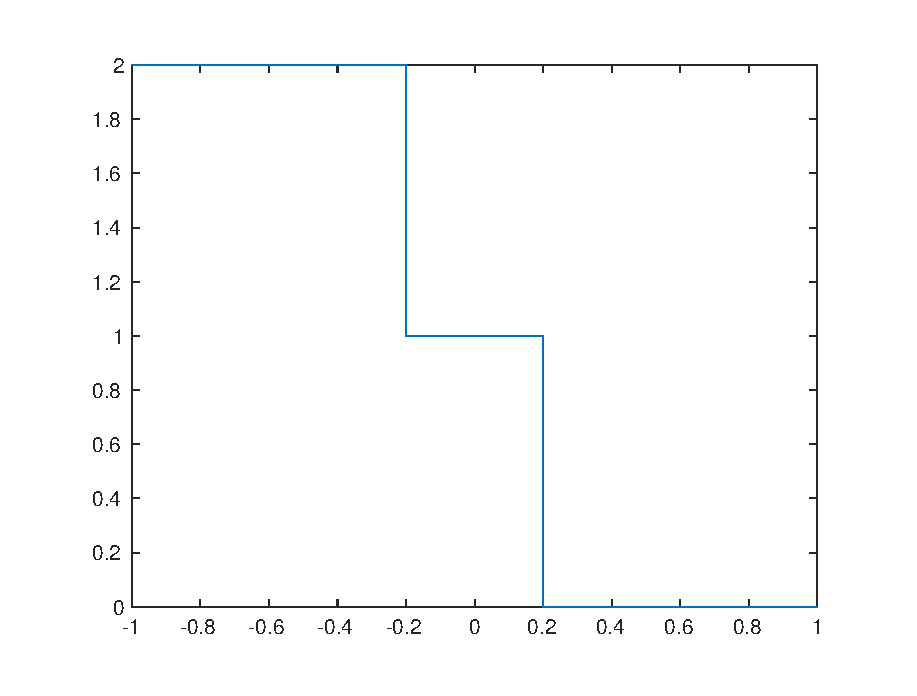
\includegraphics[width=0.45\textwidth,height=0.2\textheight]{./images/Burgers_2-1-0_t0.eps}
}
\subfigure[t=0.2]{
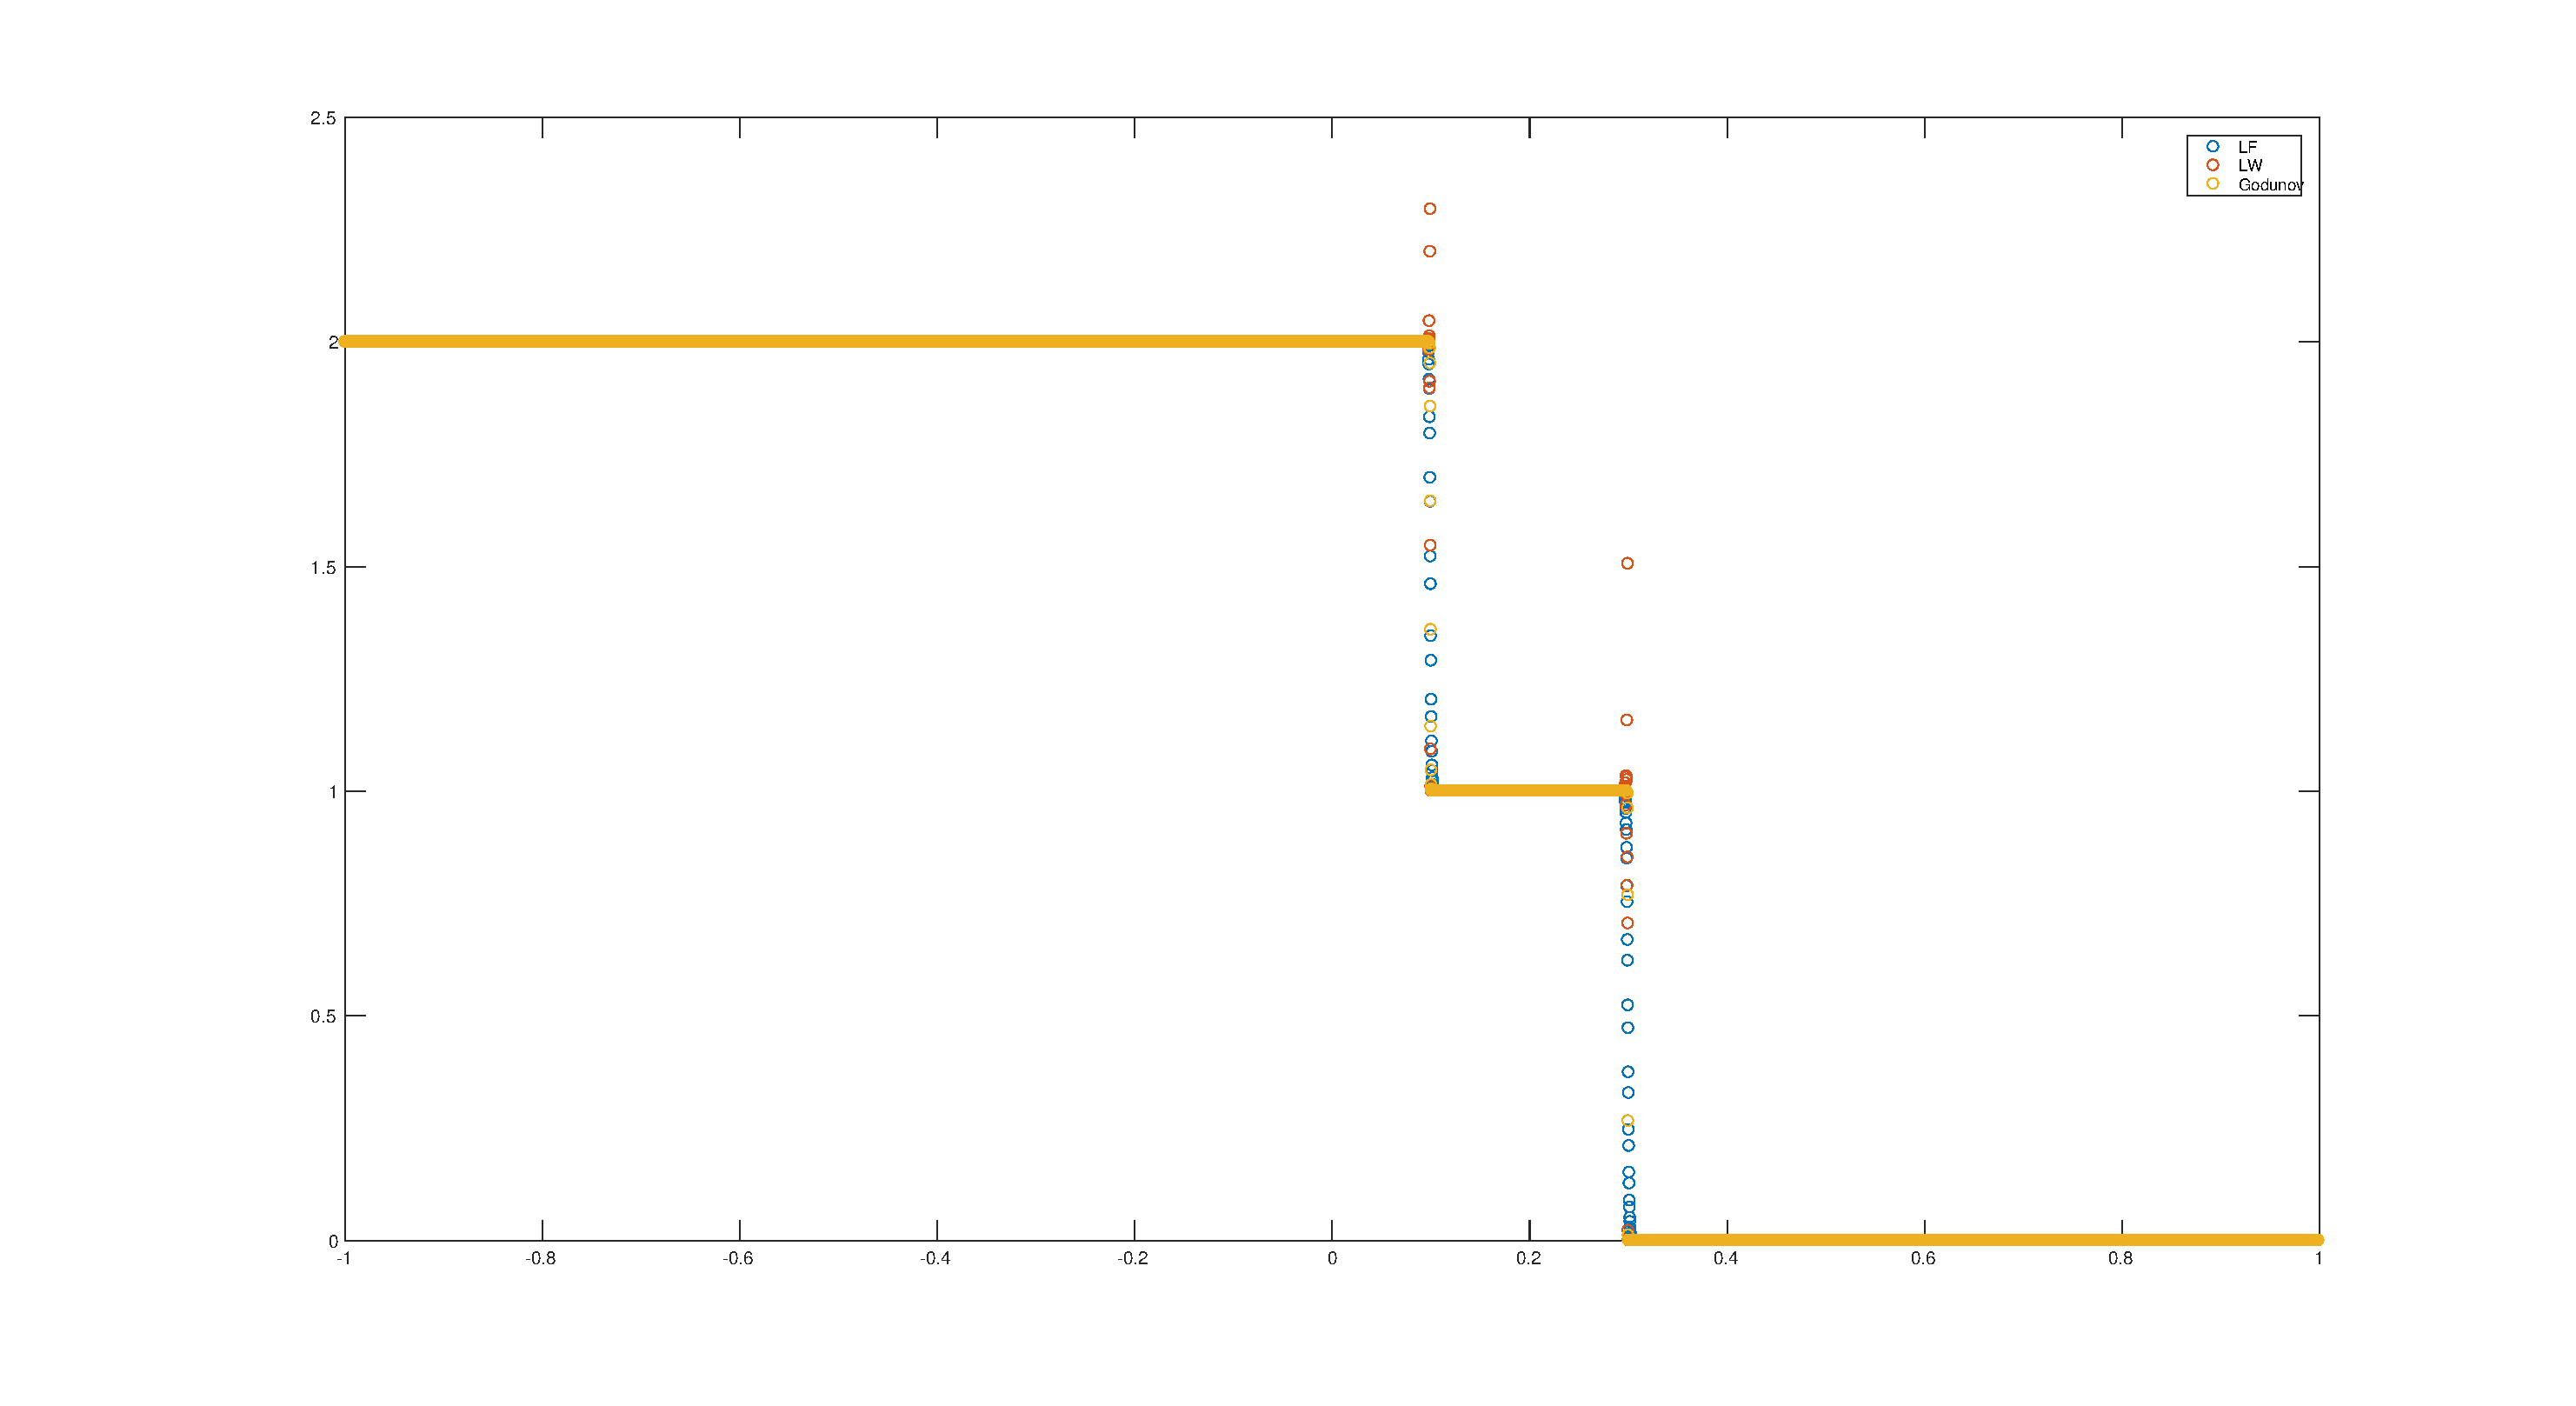
\includegraphics[width=0.45\textwidth,height=0.2\textheight]{./images/Burgers_2-1-0_tpt2.eps}
}
\subfigure[t=0.39]{
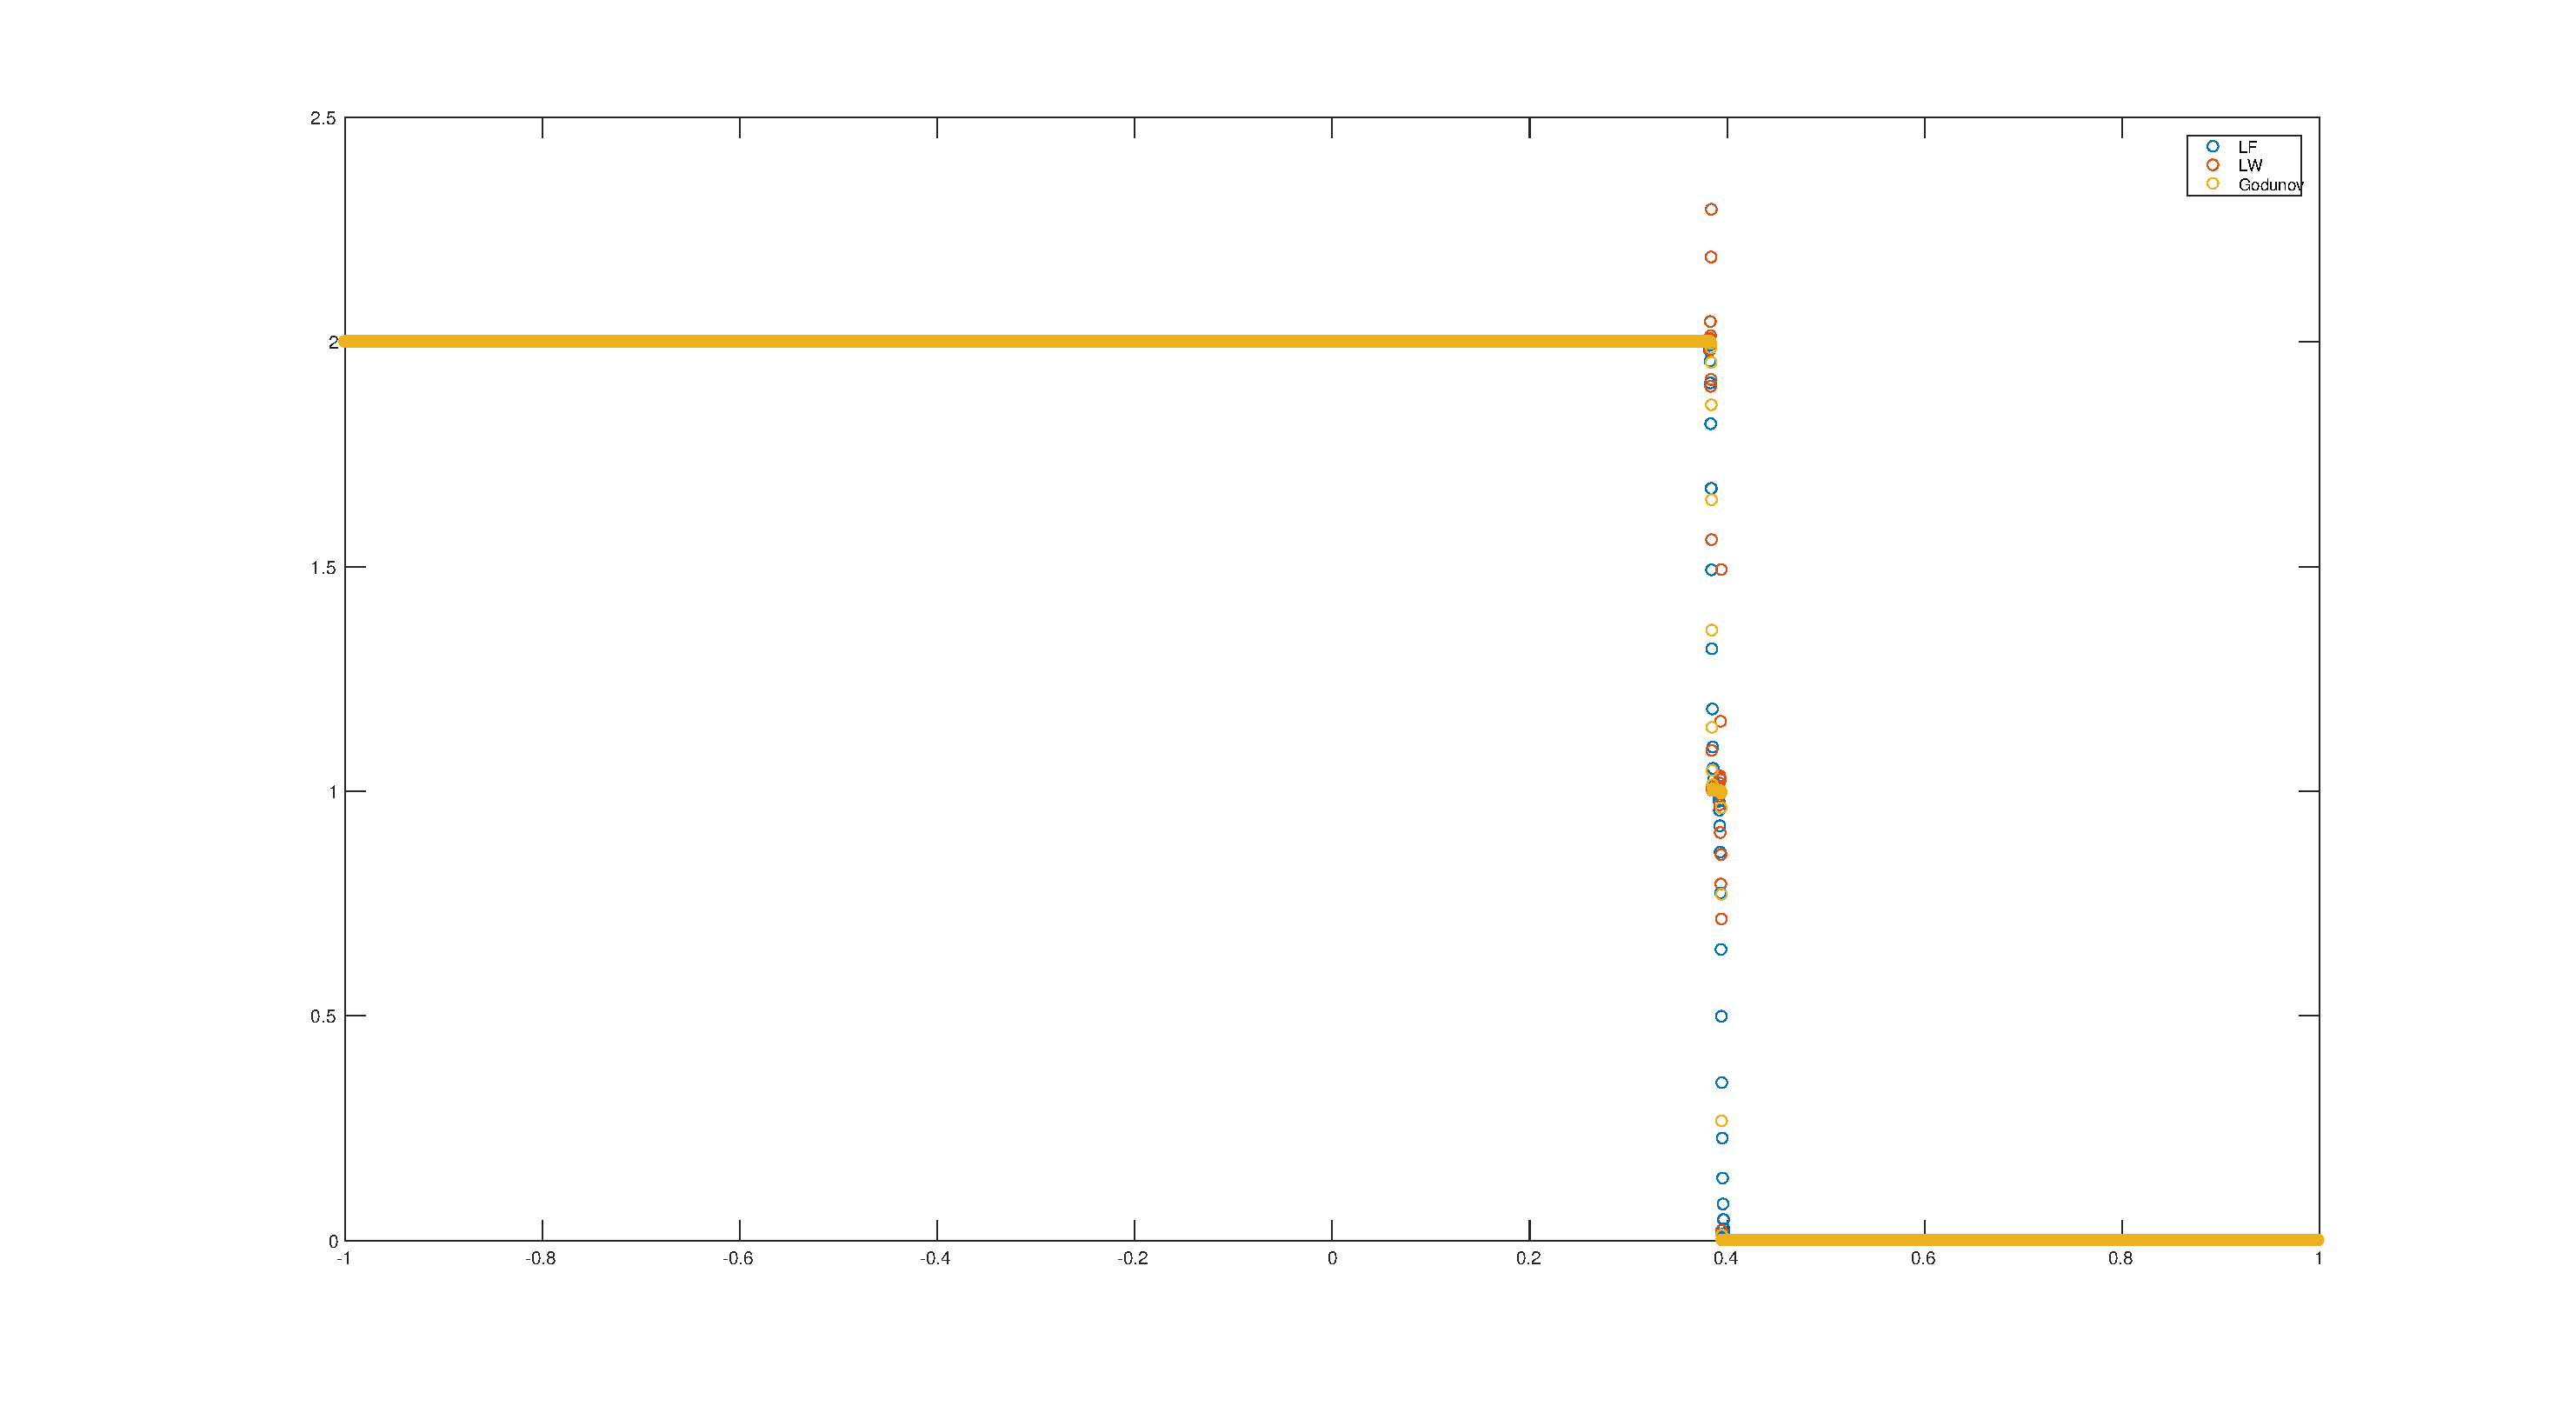
\includegraphics[width=0.45\textwidth,height=0.2\textheight]{./images/Burgers_2-1-0_tpt39.eps}
}\hspace{0.9cm}
\subfigure[t=0.5]{
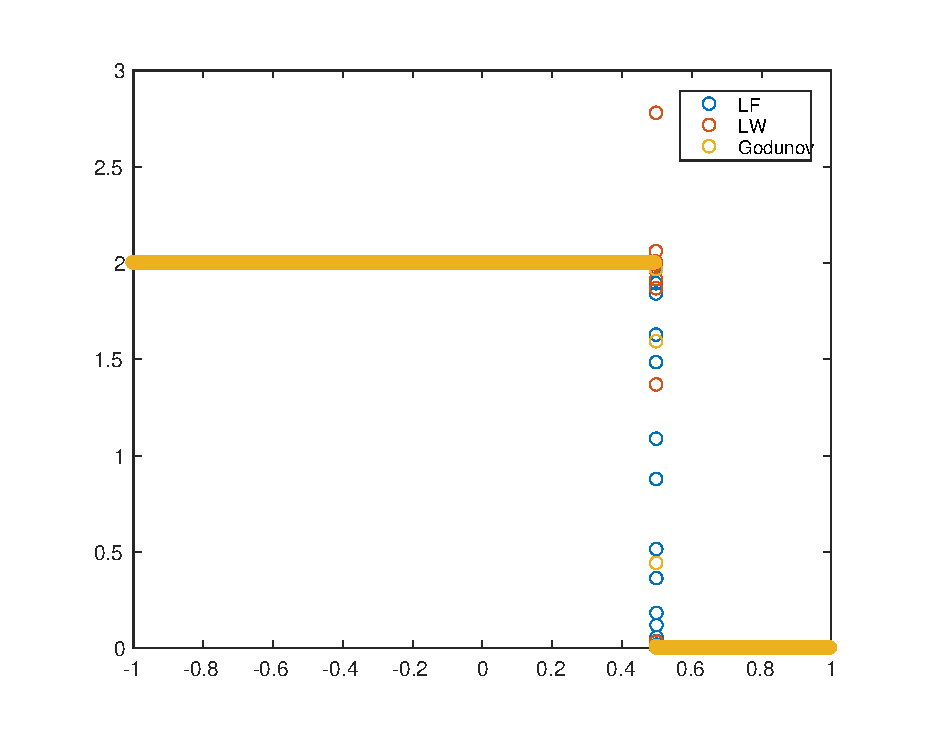
\includegraphics[width=0.45\textwidth,height=0.2\textheight]{./images/Burgers_2-1-0_tpt5.eps}
}
\end{figure}
可见初始两个激波分别独立传播,速度分别为
$\frac{2+1}{2}=1.5,\frac{1+0}{2}=0.5$,经过$t=0.4$时间之后,激波相遇合
并为一个激波,之后按照该激波速度$\frac{2+0}{2}=1$速度传播。
\subsubsection{稀疏波}
再考虑两个间断都为稀疏波的情形,即$u_l < u_m < u_r$。
我们取得初值为
\[  u_l = 0, u_m = 1, u_r = 2, x_l = -0.2 , x_r= 0.2\]
\begin{figure}[H]
  \centering  
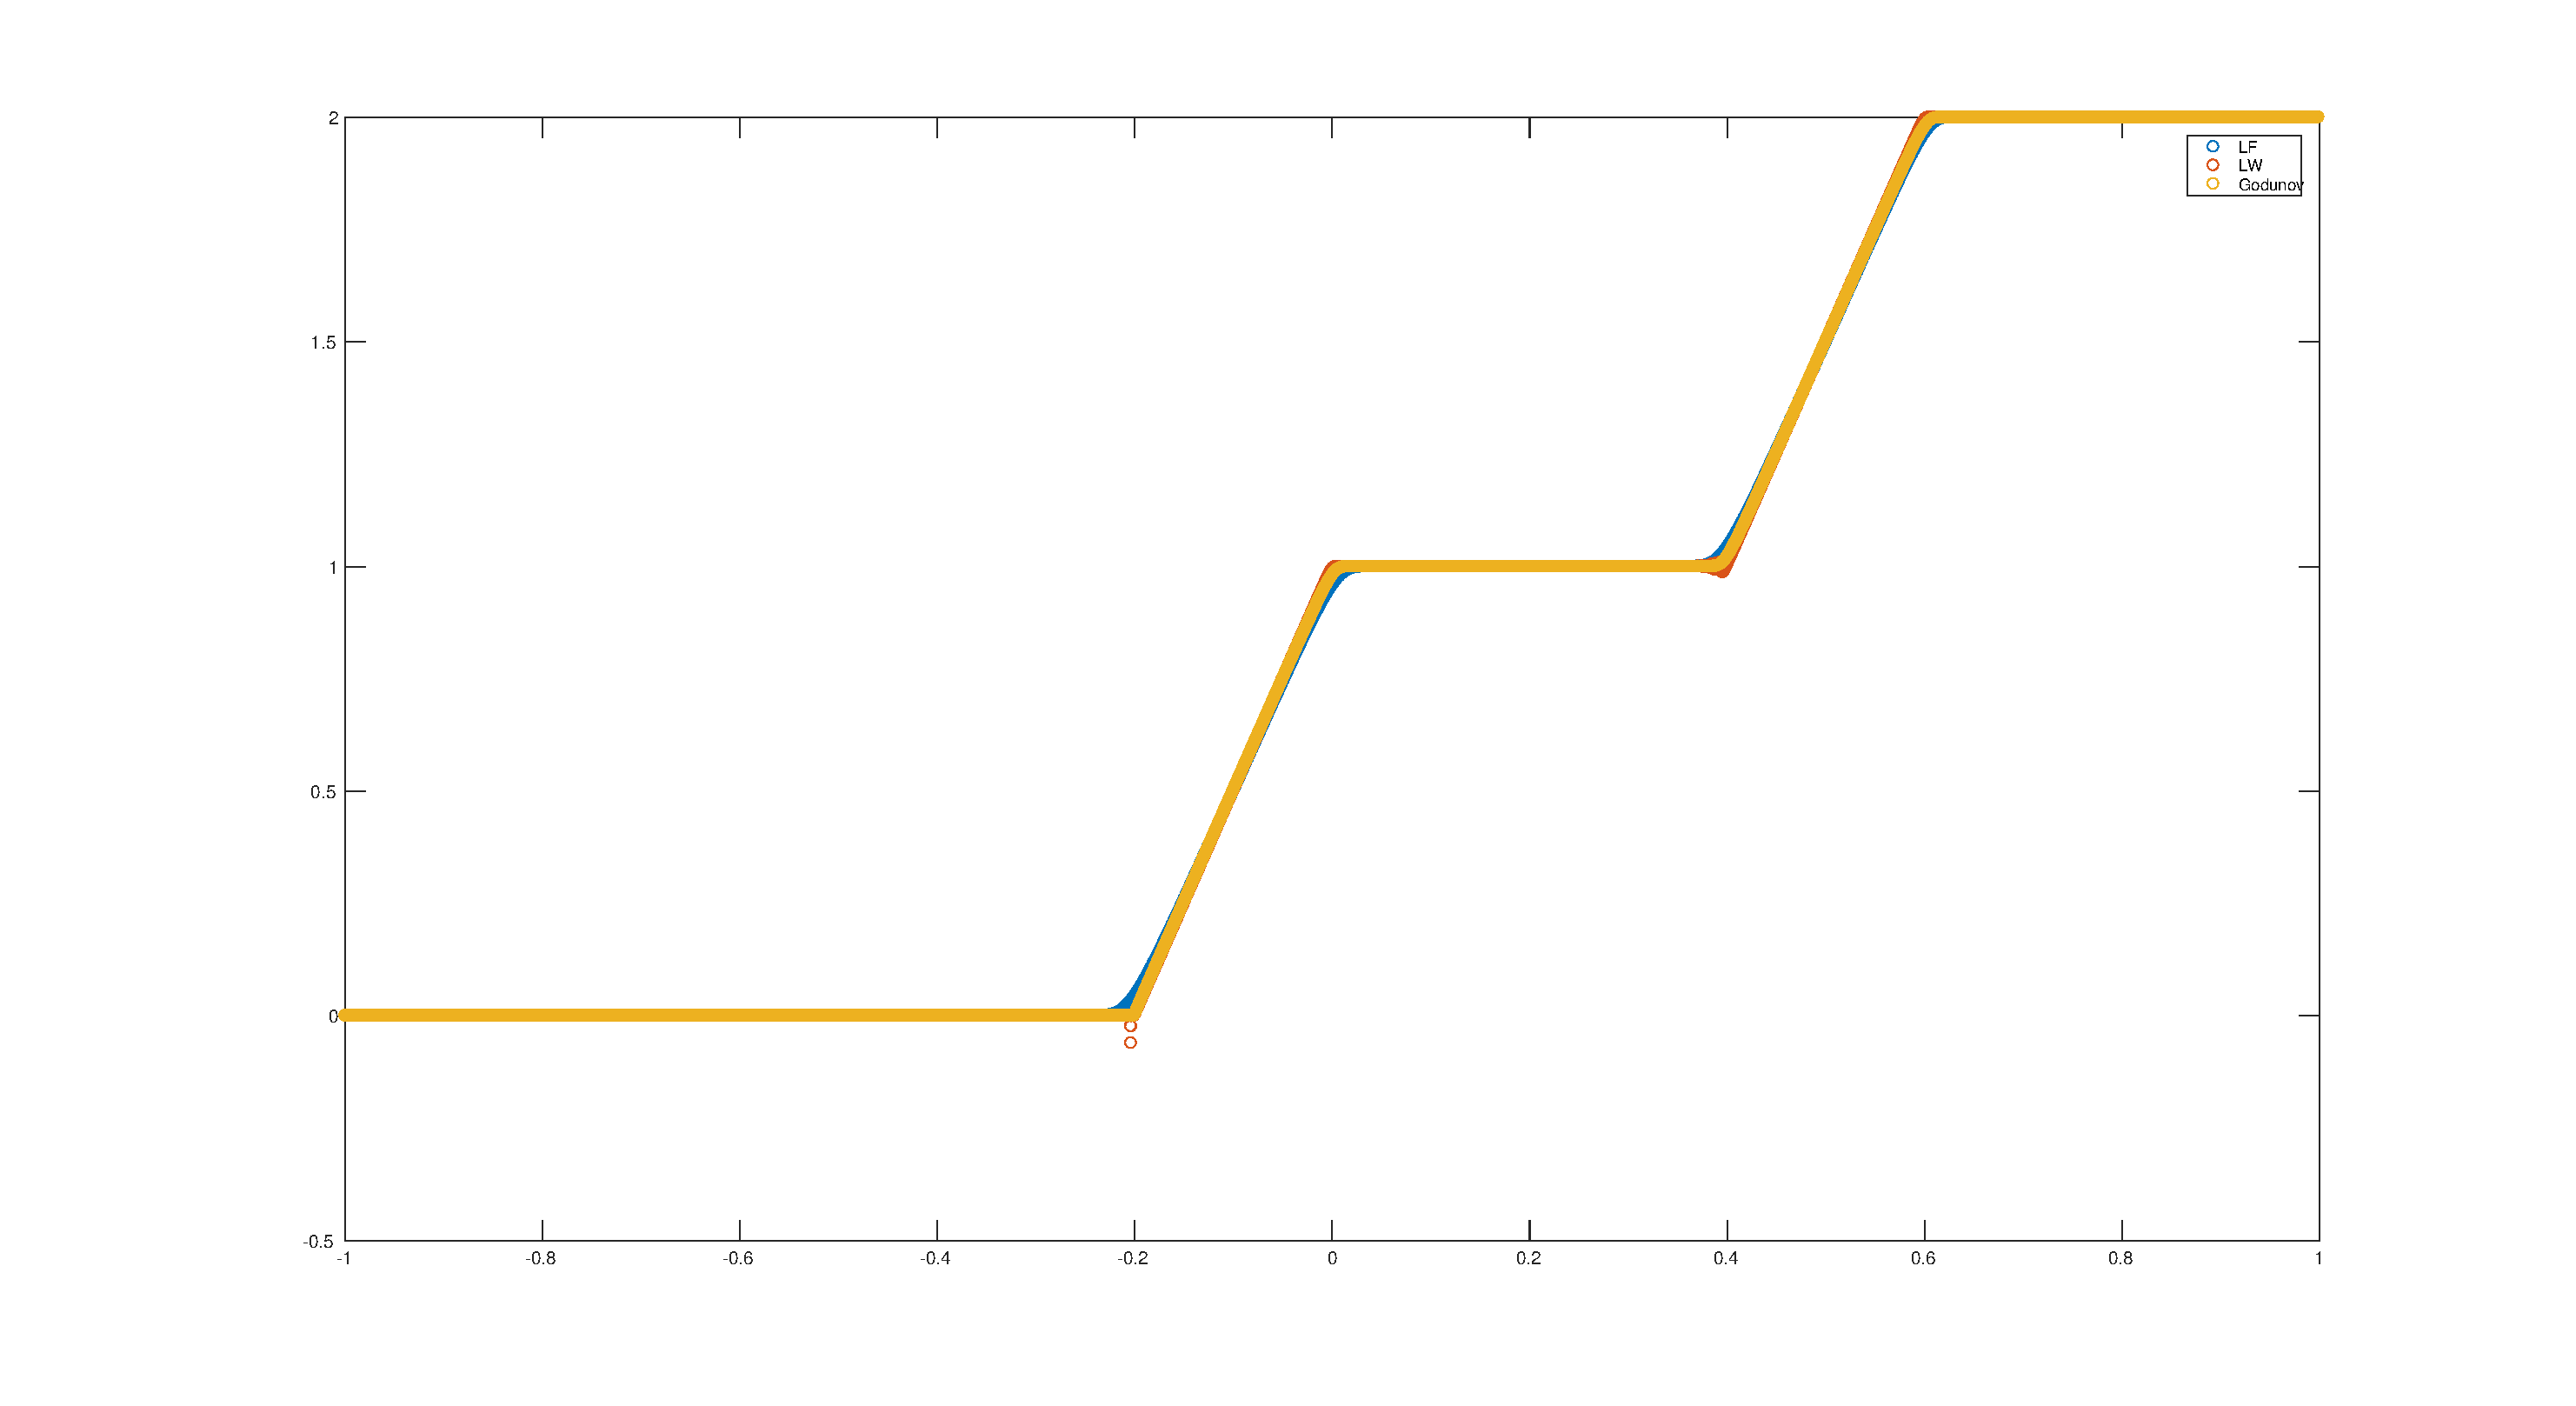
\includegraphics[width=0.9\textwidth]{./images/Burgers_0-1-2_tpt2.eps}
  \caption{稀疏波,t=0.2}
\end{figure}
可见两个稀疏波独立传播,互不干扰。
\subsubsection{激波与稀疏波的相遇}
最后考虑一个稀疏波和一个激波的情形。
我们取得初值为
\[  u_l = -1, u_m = 2, u_r = 0, x_l = -0.2 , x_r= 0.2\]
\begin{figure}[H]
\subfigure[t=0]{
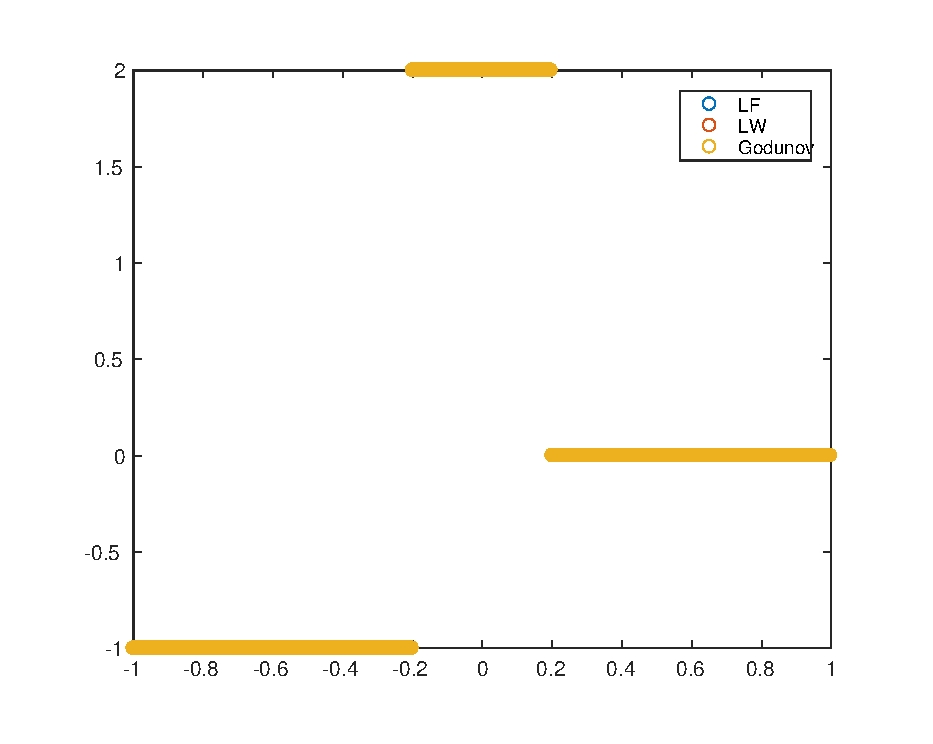
\includegraphics[width=0.45\textwidth,height=0.2\textheight]{./images/Burgers_m1-2-0_t0.eps}
}
\subfigure[t=0.2]{
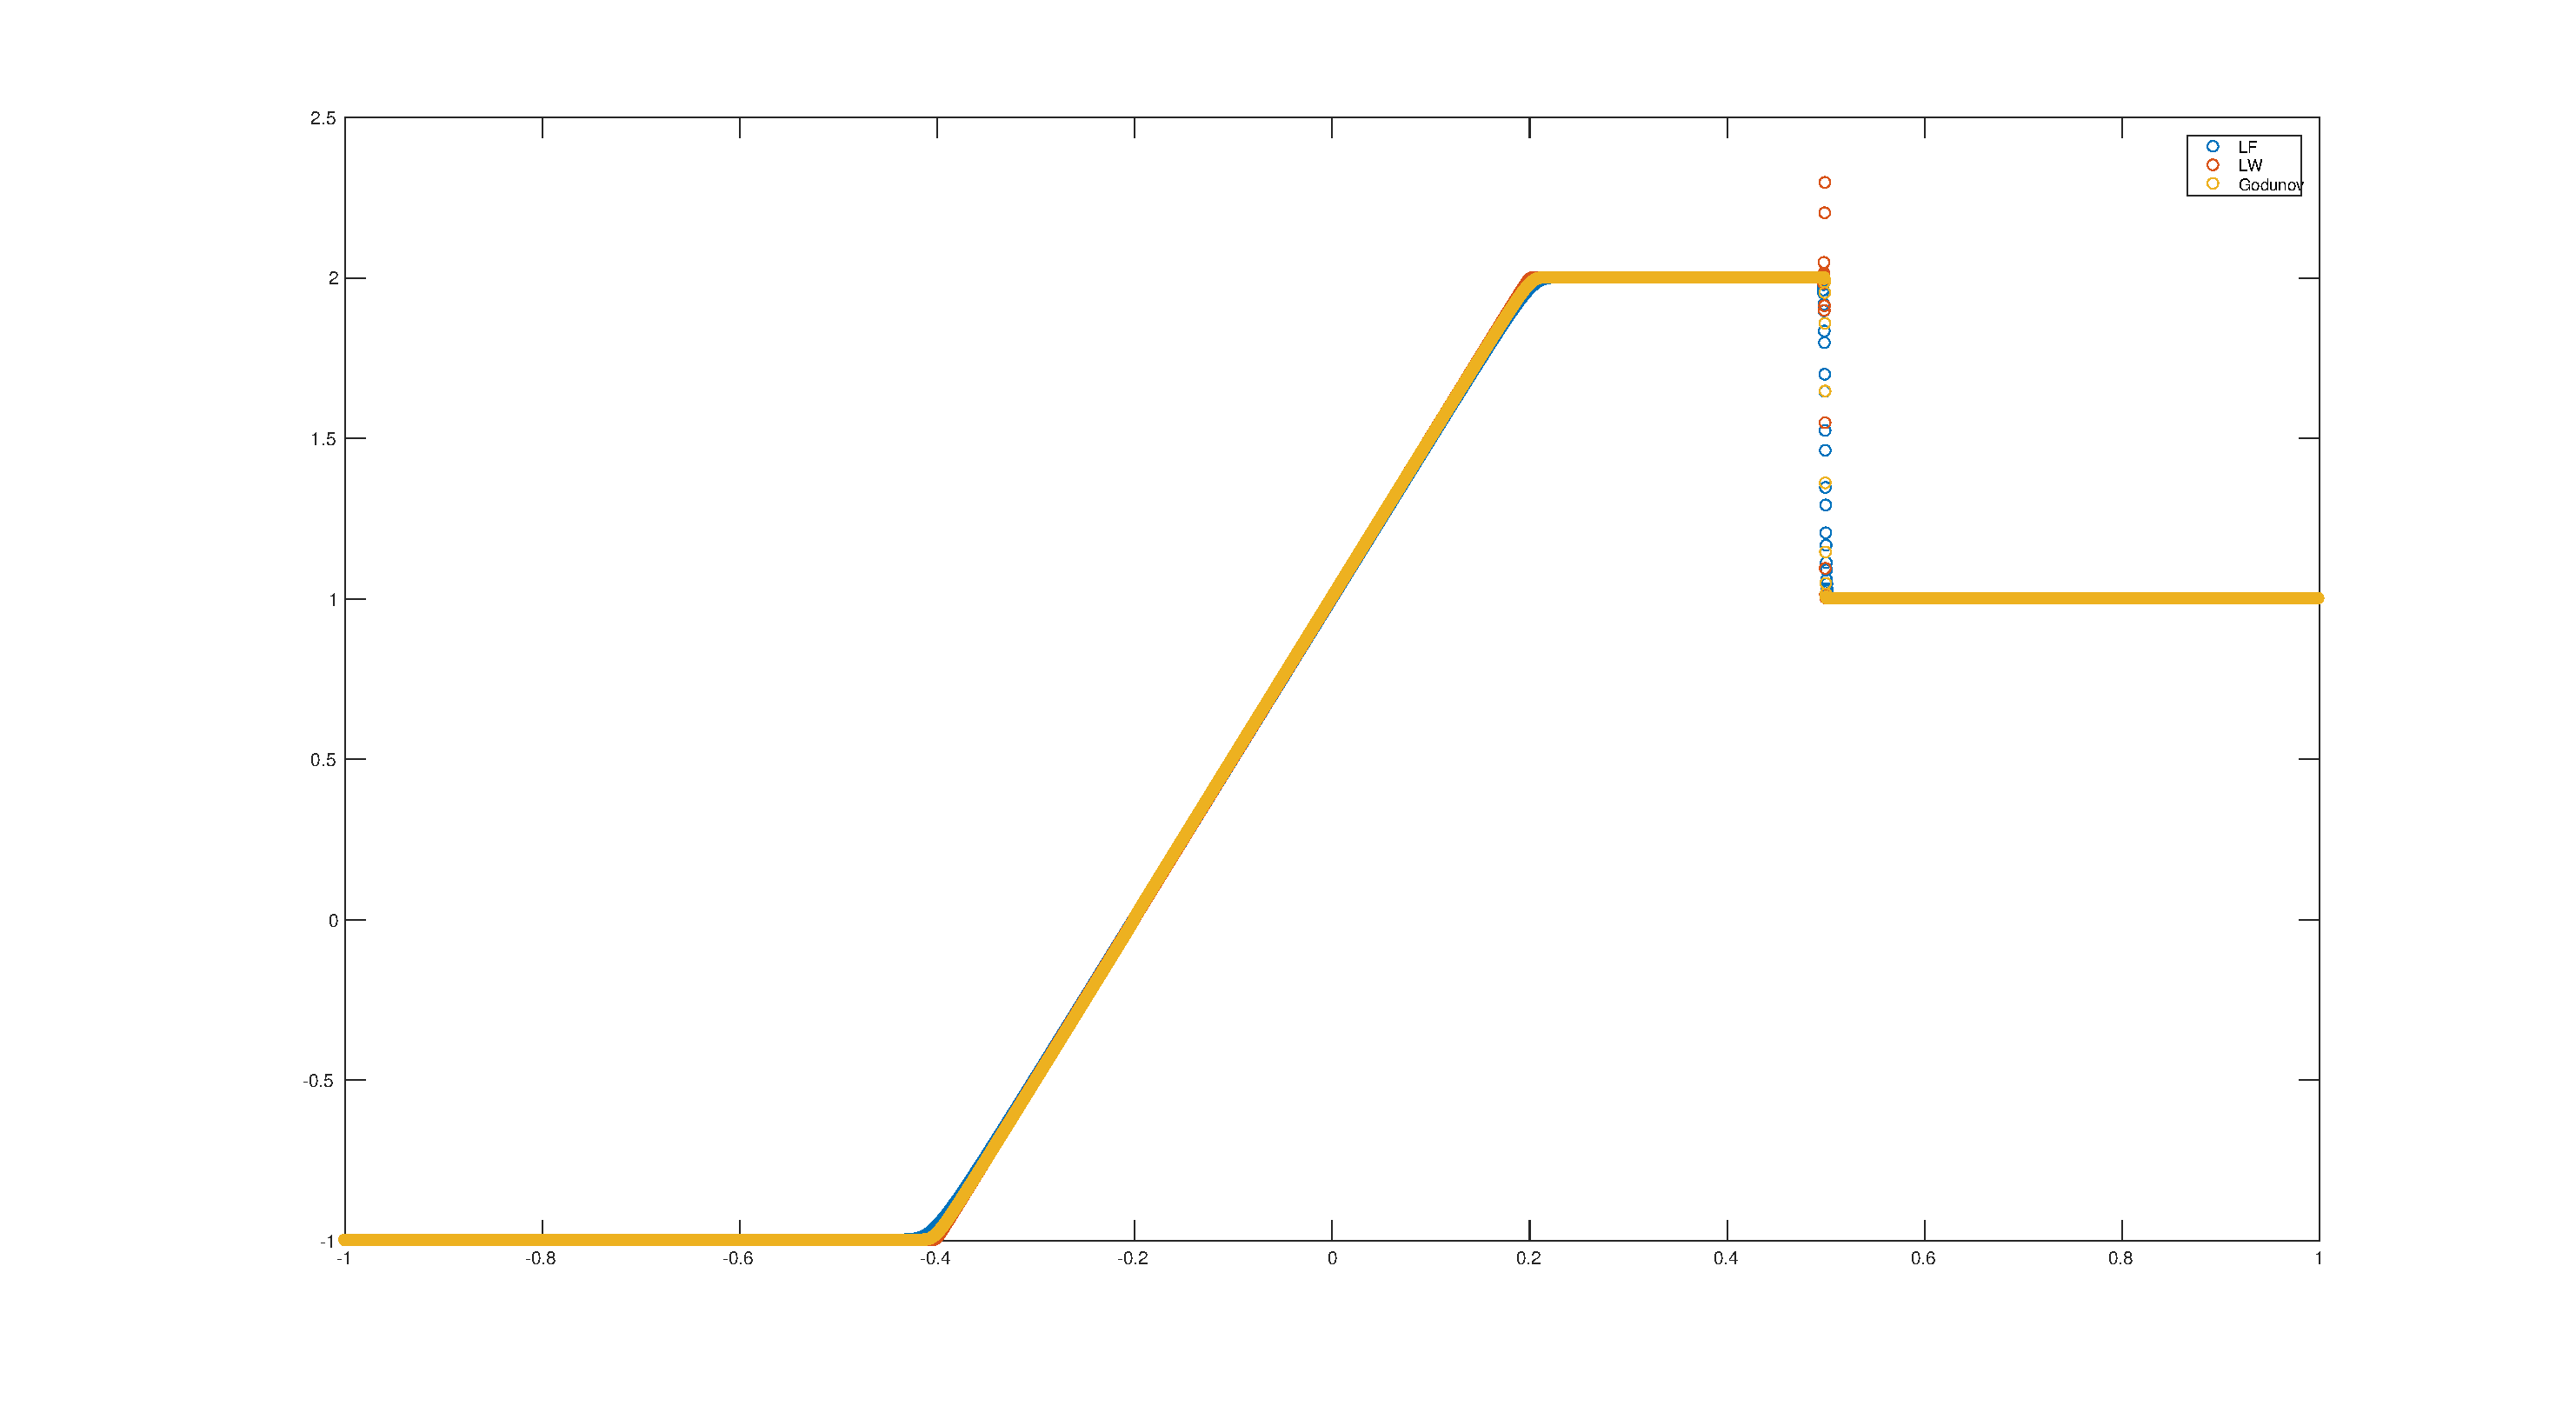
\includegraphics[width=0.45\textwidth,height=0.2\textheight]{./images/Burgers_m1-2-1_tpt2.eps}
}
\subfigure[t=0.4]{
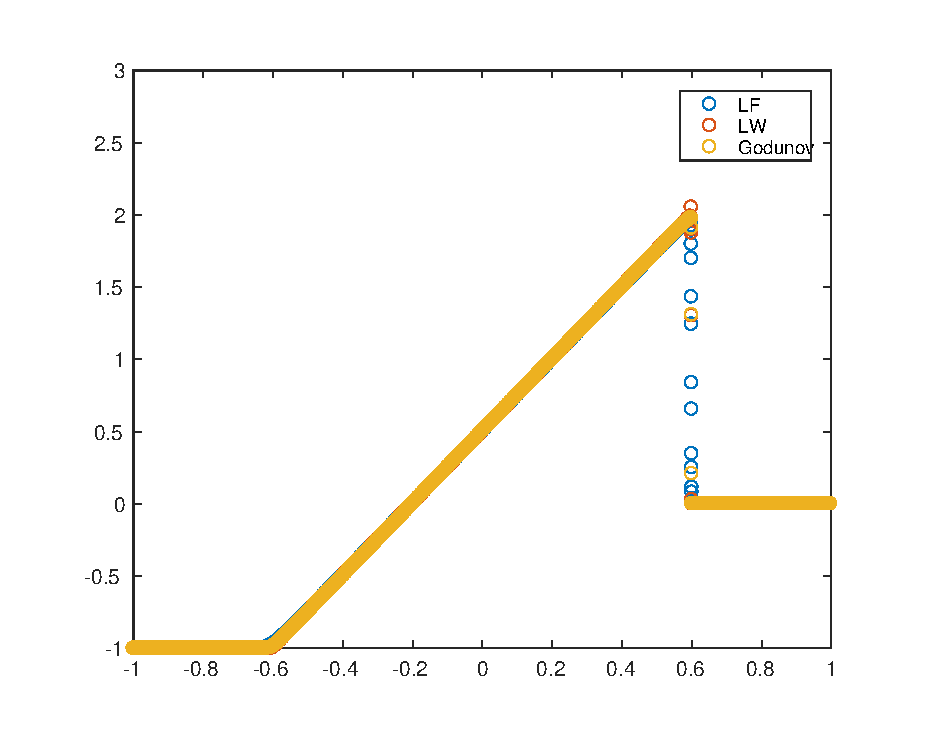
\includegraphics[width=0.45\textwidth,height=0.2\textheight]{./images/Burgers_m1-2-0_tpt4.eps}
}\hspace{0.9cm}
\subfigure[t=0.5]{
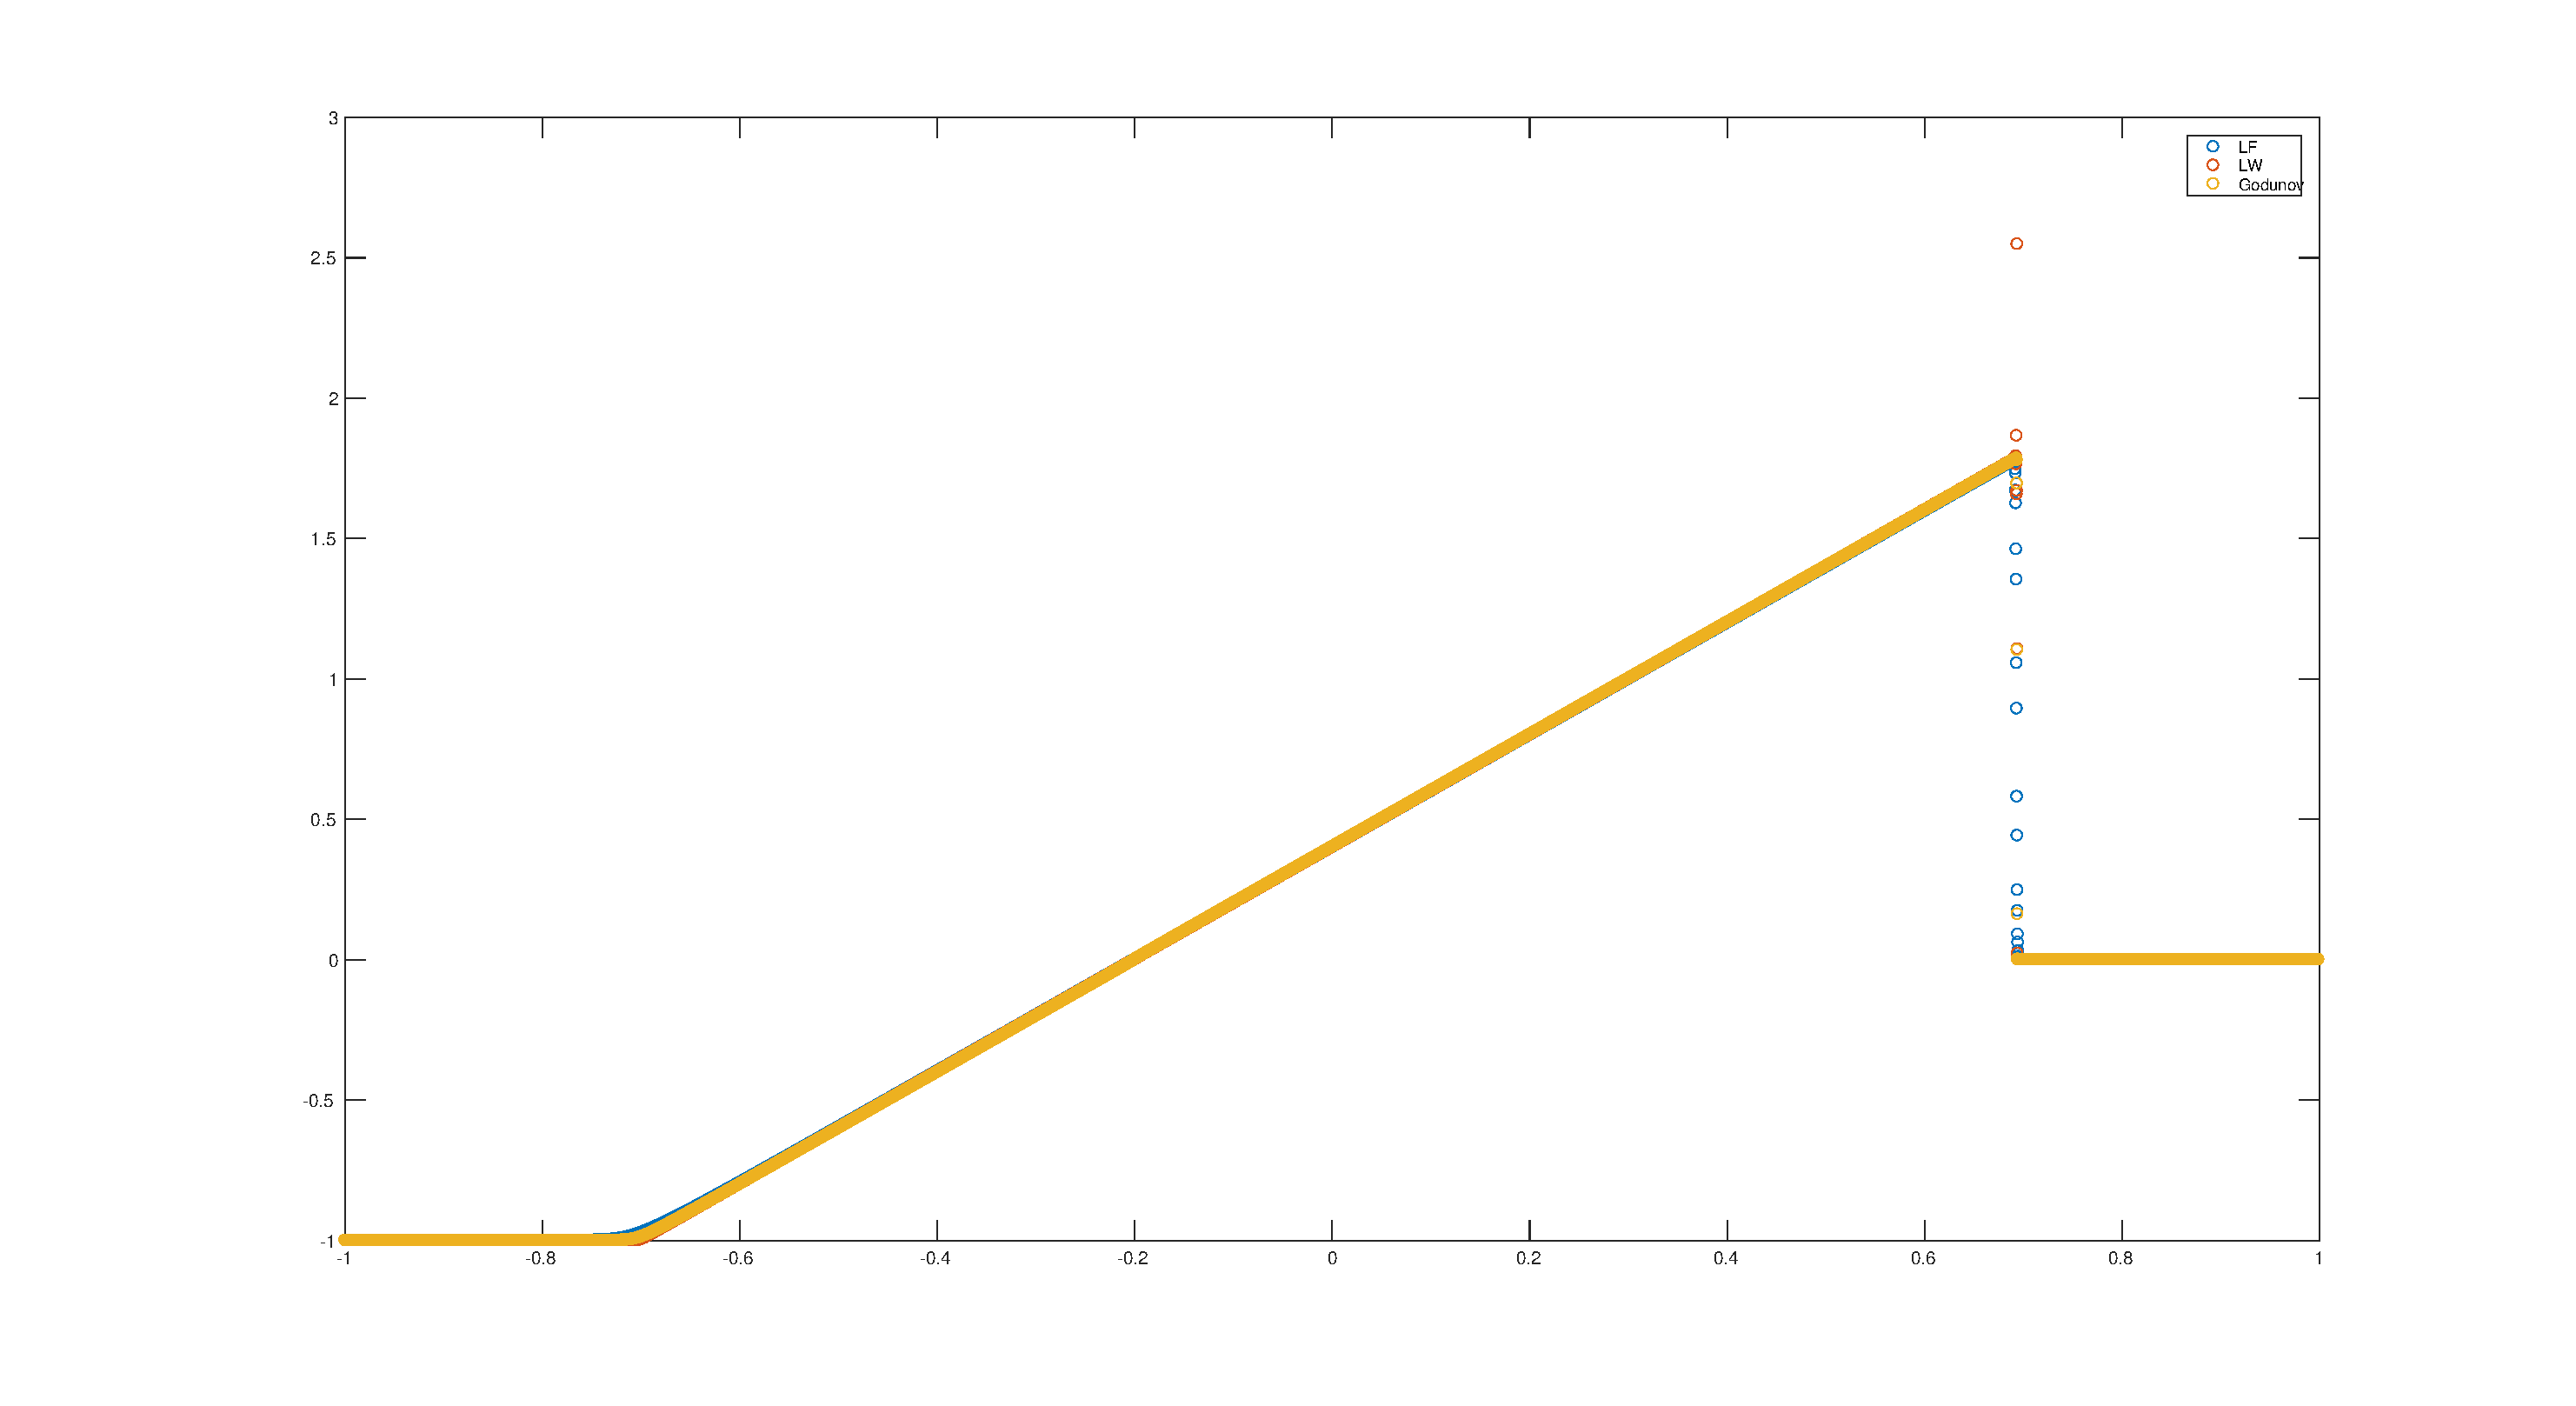
\includegraphics[width=0.45\textwidth,height=0.2\textheight]{./images/Burgers_m1-2-0_tpt5.eps}
}
\end{figure}
初始两个波独立传播,当稀疏波与激波相遇时,会出现间断,但间断左侧的值不
会保持为2,会逐渐减小。
\subsubsection{各数值通量分析}
由前文的数值实验,我们可以发现对于稀疏波,LF通量会有耗散,Godunov格式
与LW格式类似;对于激波,LW格式会出现震荡。
\section{Taylor Green Vortex Solution}
\subsection{问题描述}
\begin{equation}
  \pd{\phi}{t}+\bm v \cdot \nabla \phi=0
\end{equation}
\[  
  \bm v = \left( \sin x\cos y \exp(-2\nu t),-\cos x\sin y \exp(-2\nu
  t) \right)^T
\]
计算的区域为$[0,\pi]\times[0,\pi]$。
要考虑的初值为:
\begin{enumerate}
  \item $\phi=C-\sin x\sin y$
  \item $\phi=C-\sin(2x)\sin(2y)$
  \item
    $\phi=C-\left(x-\frac{\pi}{2}\right)^2\left(y-\frac{\pi}{2}\right)^2$
\end{enumerate}
\subsection{算法分析}
该方程可以写成守恒型格式
\[  
\pd{\phi}{t} + \nabla \cdot \bm{F} = 0
 \]
 其中$\bm F=(\sin x\cos y\exp(-2\nu t)\phi,
 -\cos x\sin y\exp(-2\nu
 t)\phi)^T$
 利用守恒型差分格式,
 \[ 
 \phi^{m+1}_{i,j}=\phi_{i,j}^m
 -\frac{\Delta t}{\Delta
 x}\left(F_{i+\frac 12,j}^{m+\frac 12}-F_{i-\frac 12,j}^{m+\frac
 12}\right)
 -\frac{\Delta t}{\Delta
 y}\left(G_{i,j+\frac 12}^{m+\frac 12}-G_{i,j-\frac 12}^{m+\frac
 12}\right)
 \]
\subsection{数值结果}
\subsection{初值1}
对于初值
\[  
  \phi=1-\sin x\sin y
\]
计算时取$\nu=0$,$N=100,t_{end}=2$,结果如下:

\begin{figure}[H]
\subfigure[Upwind]{
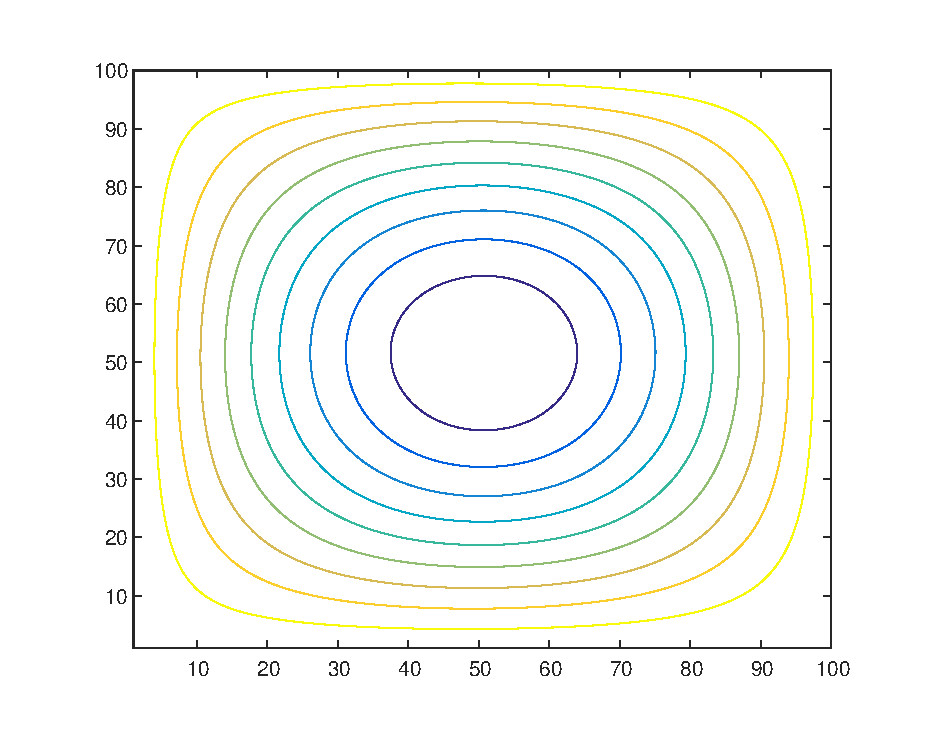
\includegraphics[width=0.45\textwidth,height=0.2\textheight]{./images/UW1.eps}
}
\subfigure[WENO]{
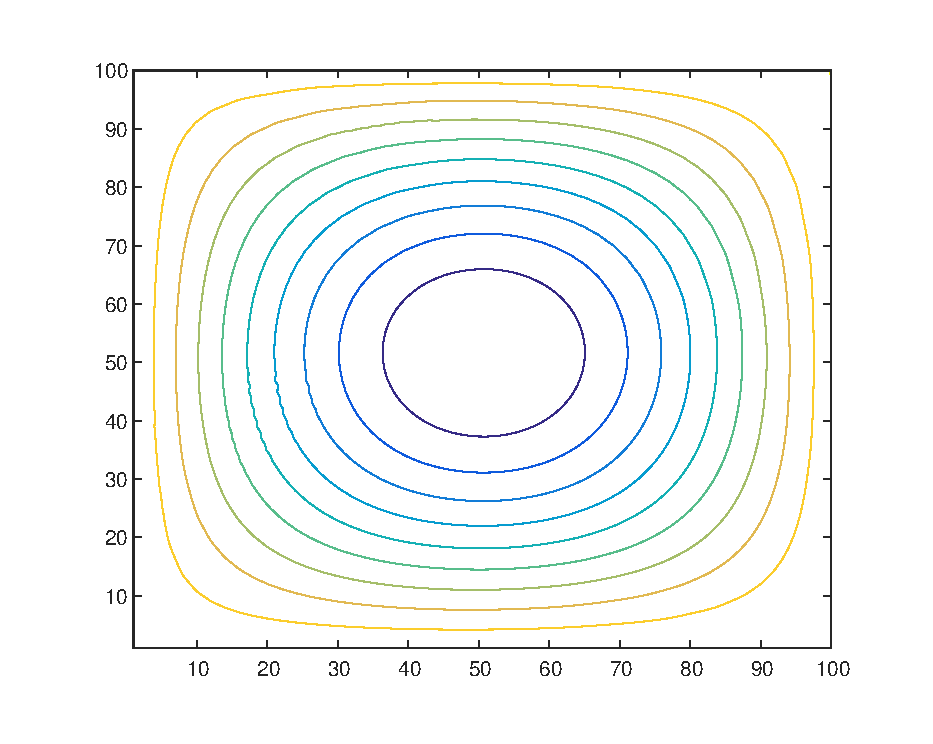
\includegraphics[width=0.45\textwidth,height=0.2\textheight]{./images/WENO1.eps}
}
\end{figure}
将$320\times 320$网格的解作为参考解,得到的2范数误差为
\begin{table}[H]
  \centering
  \begin{tabular}{cccc}
    $N$ & 40 & 80 & 160 \\
    \hline
    Upwind &0.0160&0.0078&0.0035 \\
    order& & 1.04 &1.17 \\
    WENO5 & 0.0160 &0.0078&0.0035 \\
    order& & 1.03&1.16 \\
  \end{tabular}
\end{table}
\subsection{初值2}
对于初值
\[
  \phi = 1-\sin(2x)\sin(2y)
\]
计算时取$\nu=0.1,N=100,t_{end}=2$,结果如下:
\begin{figure}[H]
\subfigure[Upwind]{
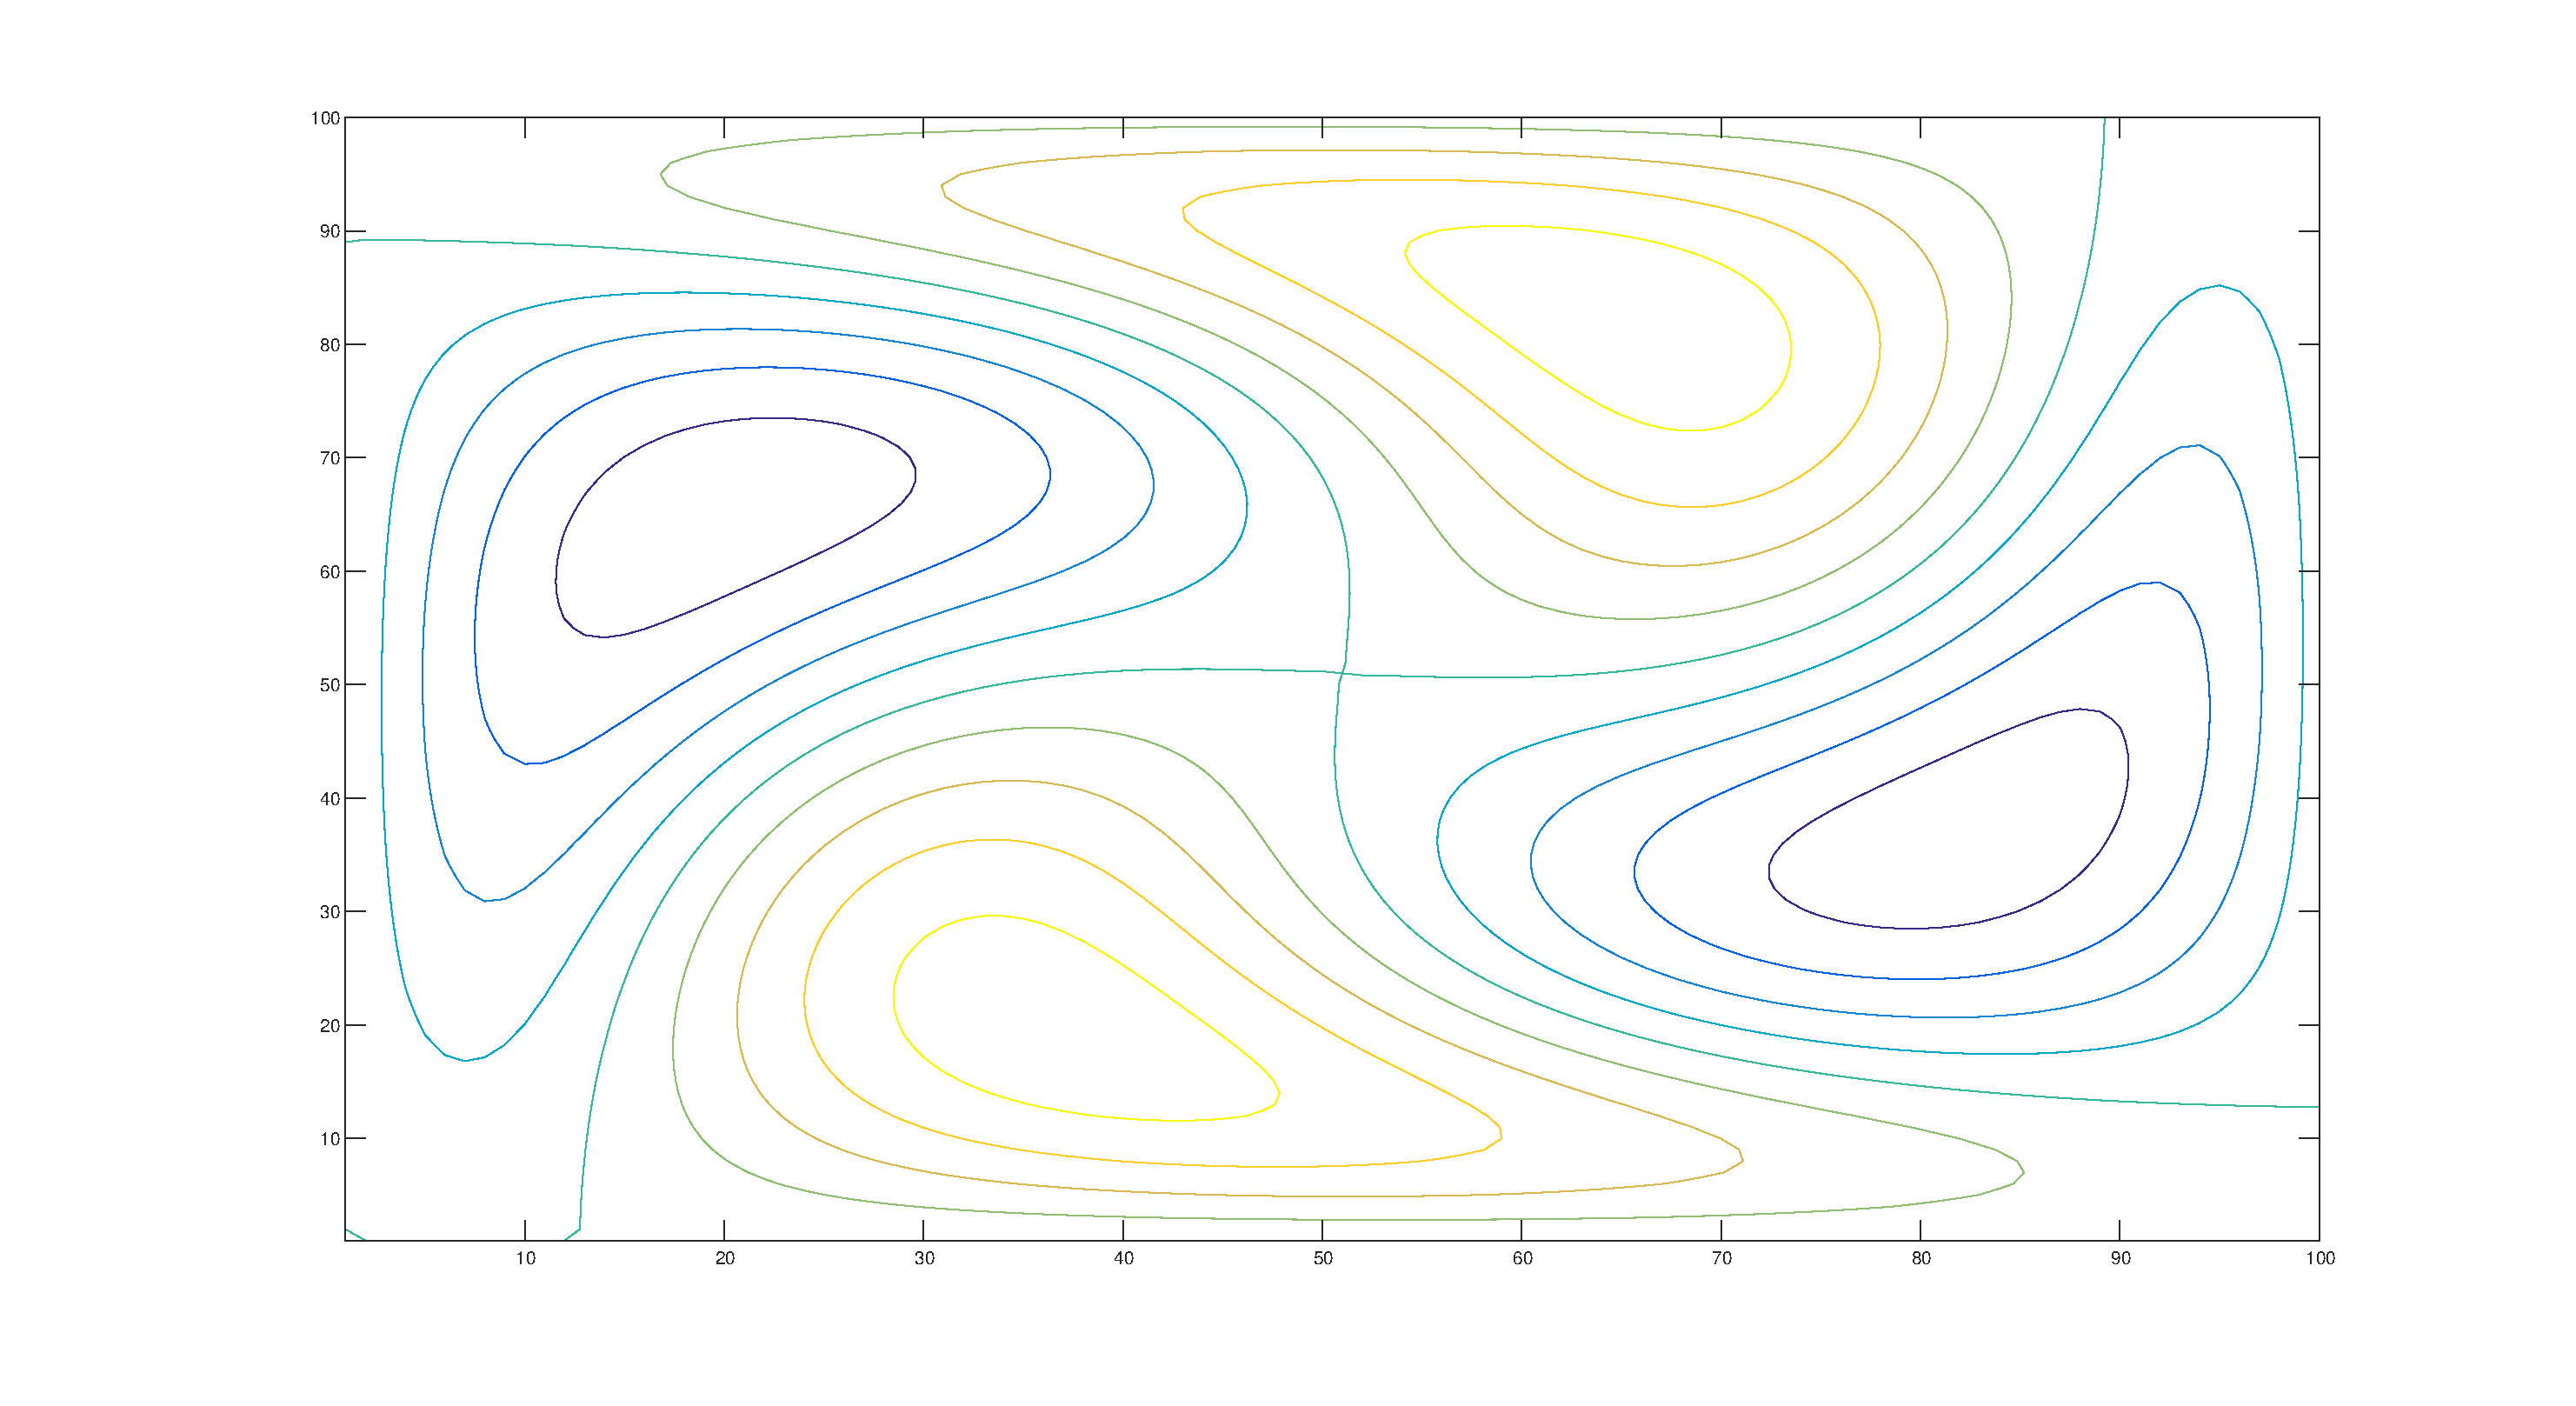
\includegraphics[width=0.45\textwidth,height=0.2\textheight]{./images/UW2.eps}
}
\subfigure[WENO]{
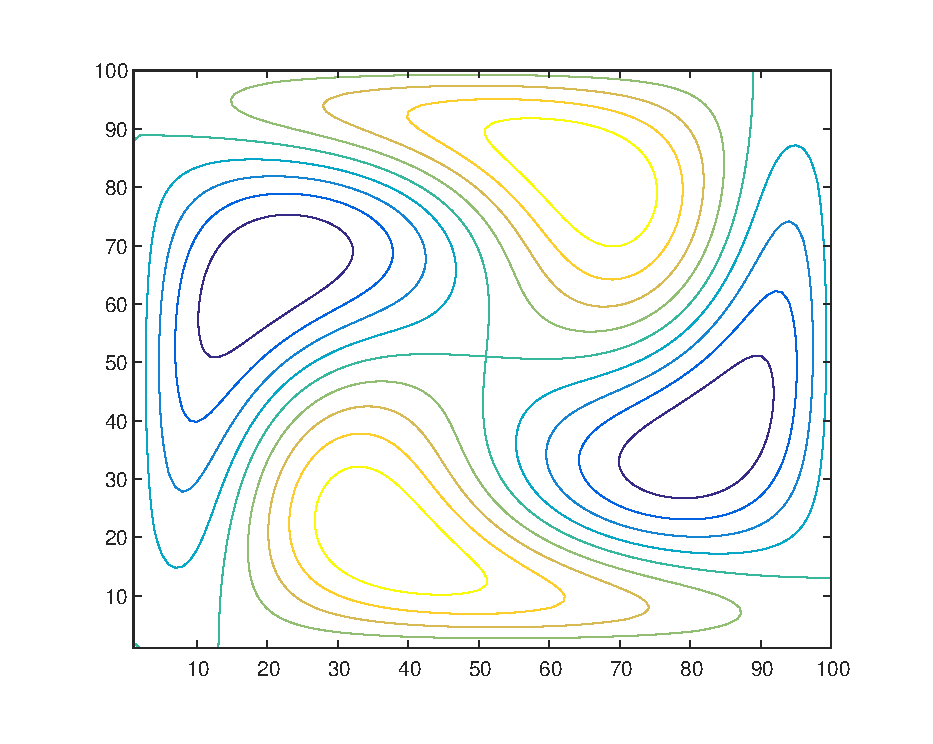
\includegraphics[width=0.45\textwidth,height=0.2\textheight]{./images/WENO2.eps}
}
\end{figure}
将$320\times 320$网格的解作为参考解,得到的2范数误差为
\begin{table}[H]
  \centering
  \begin{tabular}{cccc}
    $N$ & 40 & 80 & 160 \\
    \hline
    Upwind &0.0580&0.0260&0.0098 \\
    order& & 1.15 &1.40 \\
    WENO5 & 0.0581 &0.0260&0.098 \\
    order& & 1.16&1.40 \\
  \end{tabular}
\end{table}
\subsection{初值3}
对于初值
\[
\phi=C-\left(x-\frac{\pi}{2}\right)^2\left(y-\frac{\pi}{2}\right)^2
\]
计算时取$\nu=0.1,N=100,t_{end}=2$,结果如下:
\begin{figure}[H]
\subfigure[Upwind]{
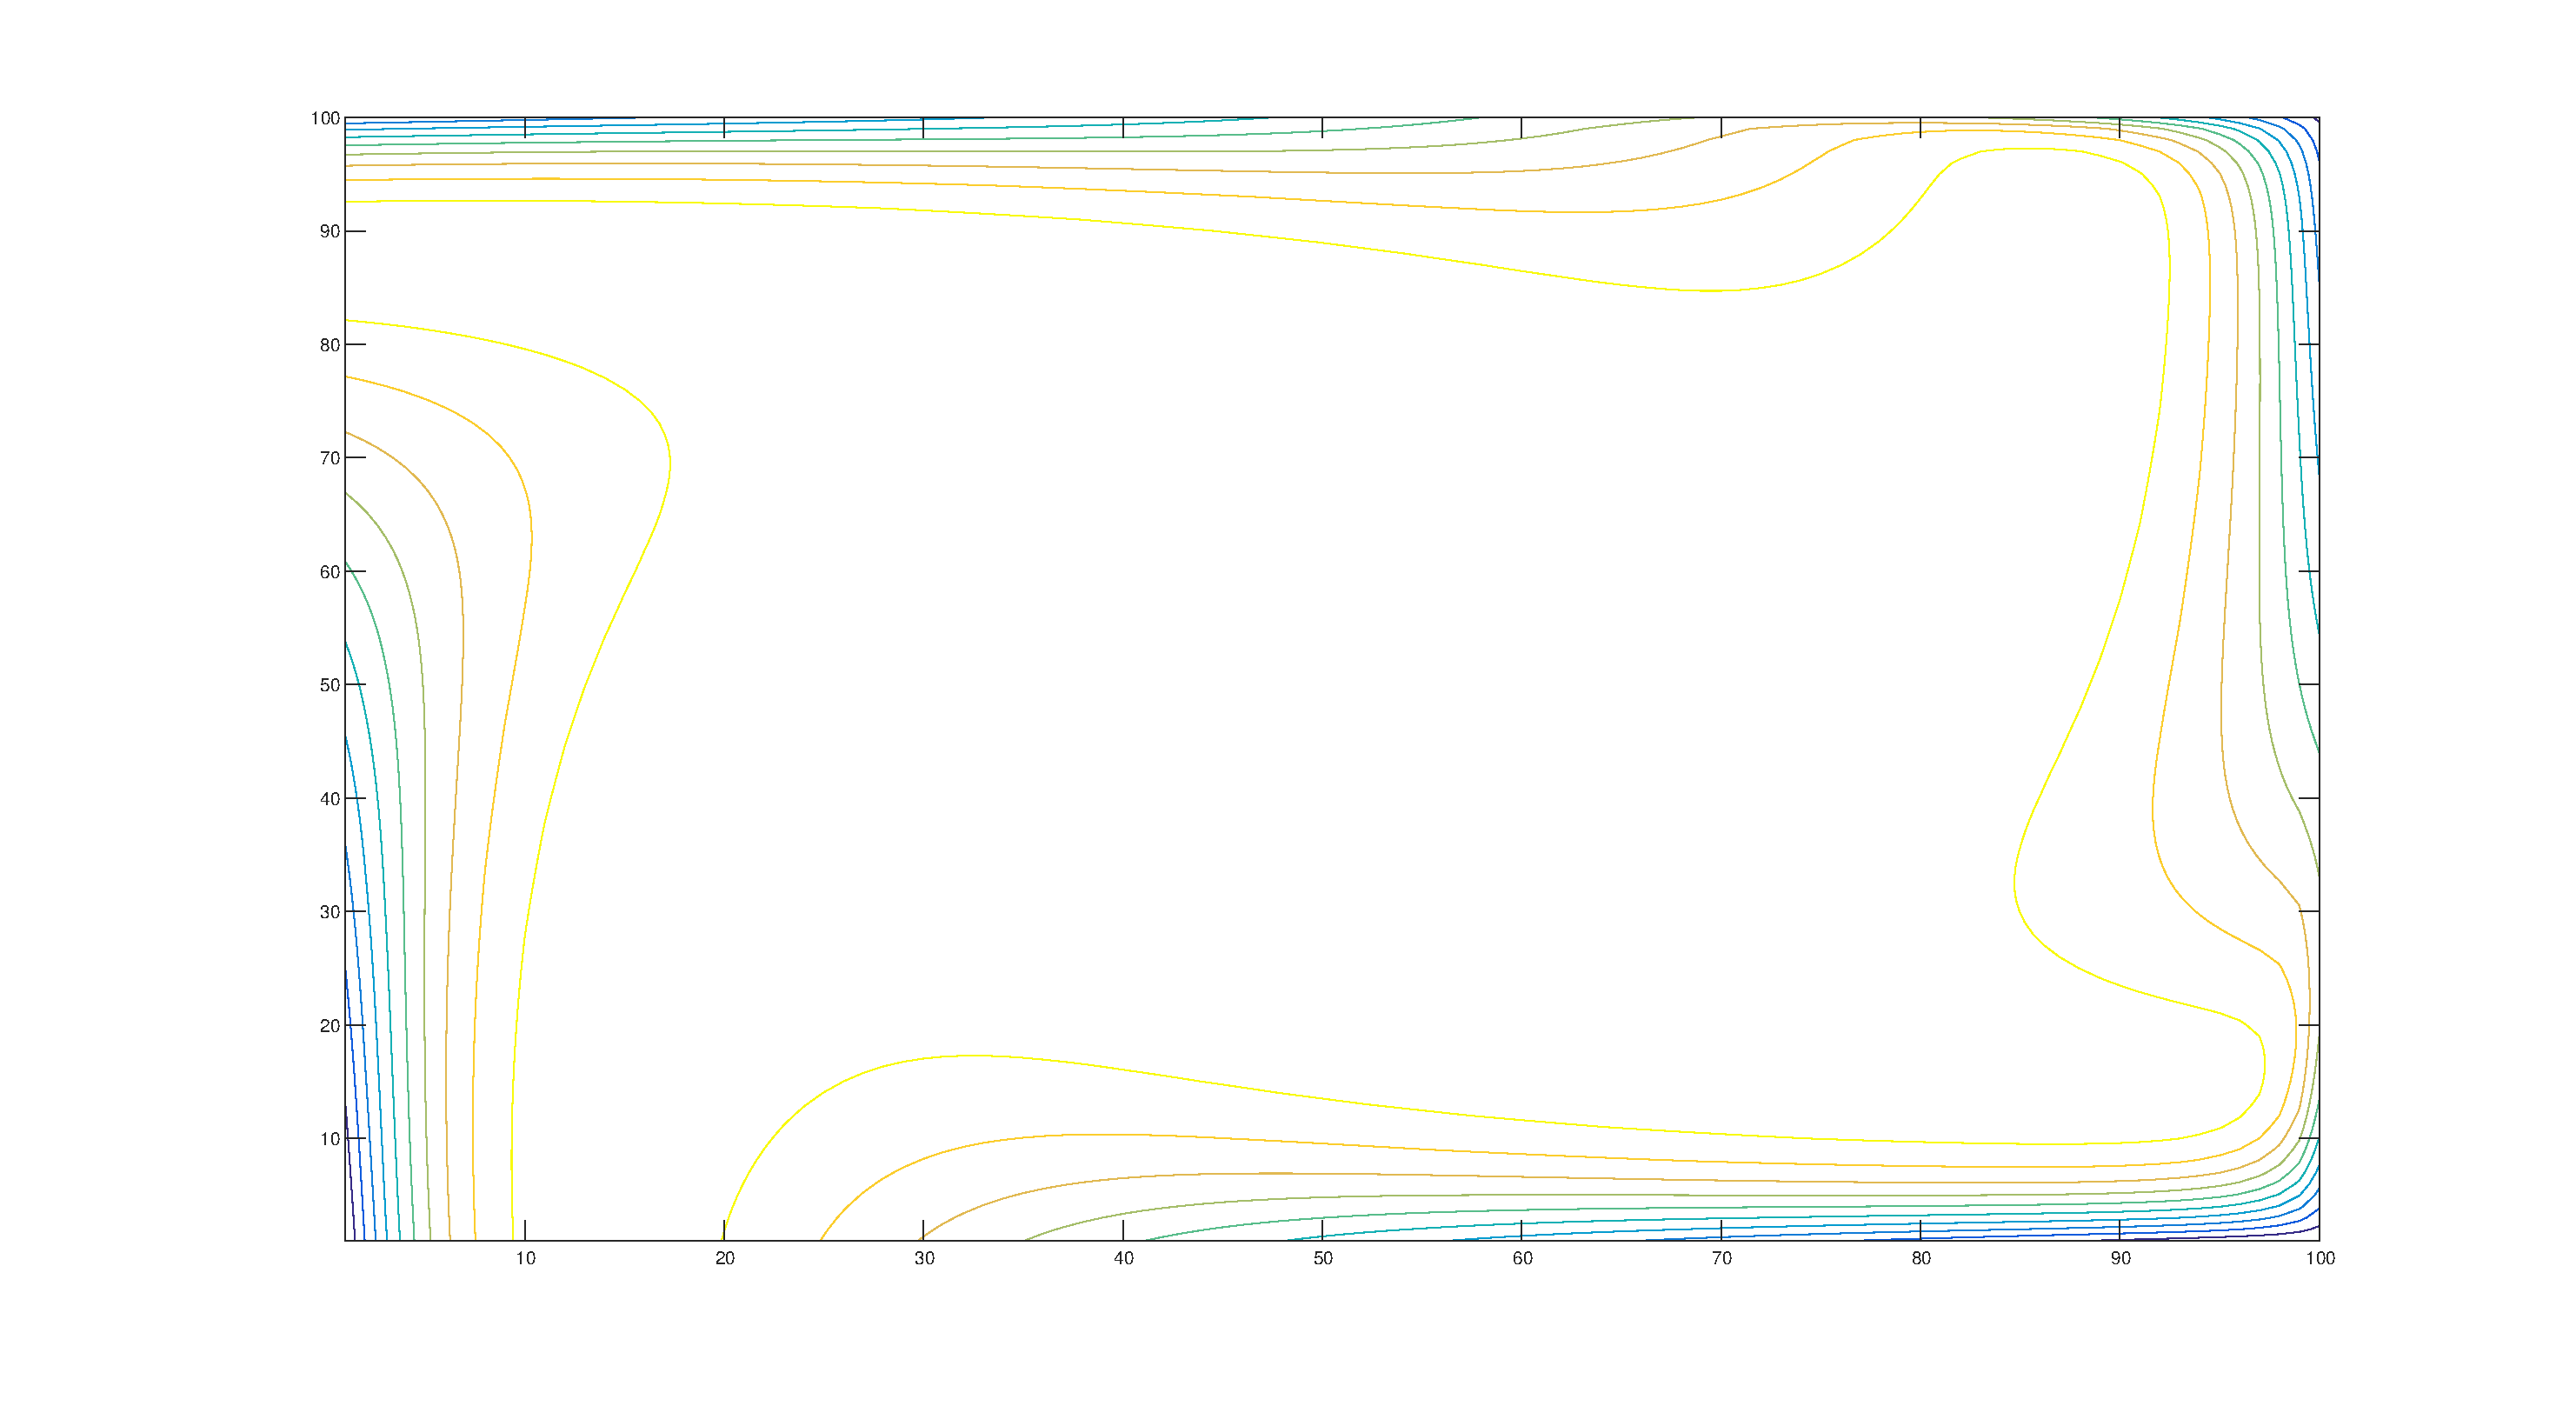
\includegraphics[width=0.45\textwidth,height=0.2\textheight]{./images/UW3.eps}
}
\subfigure[WENO]{
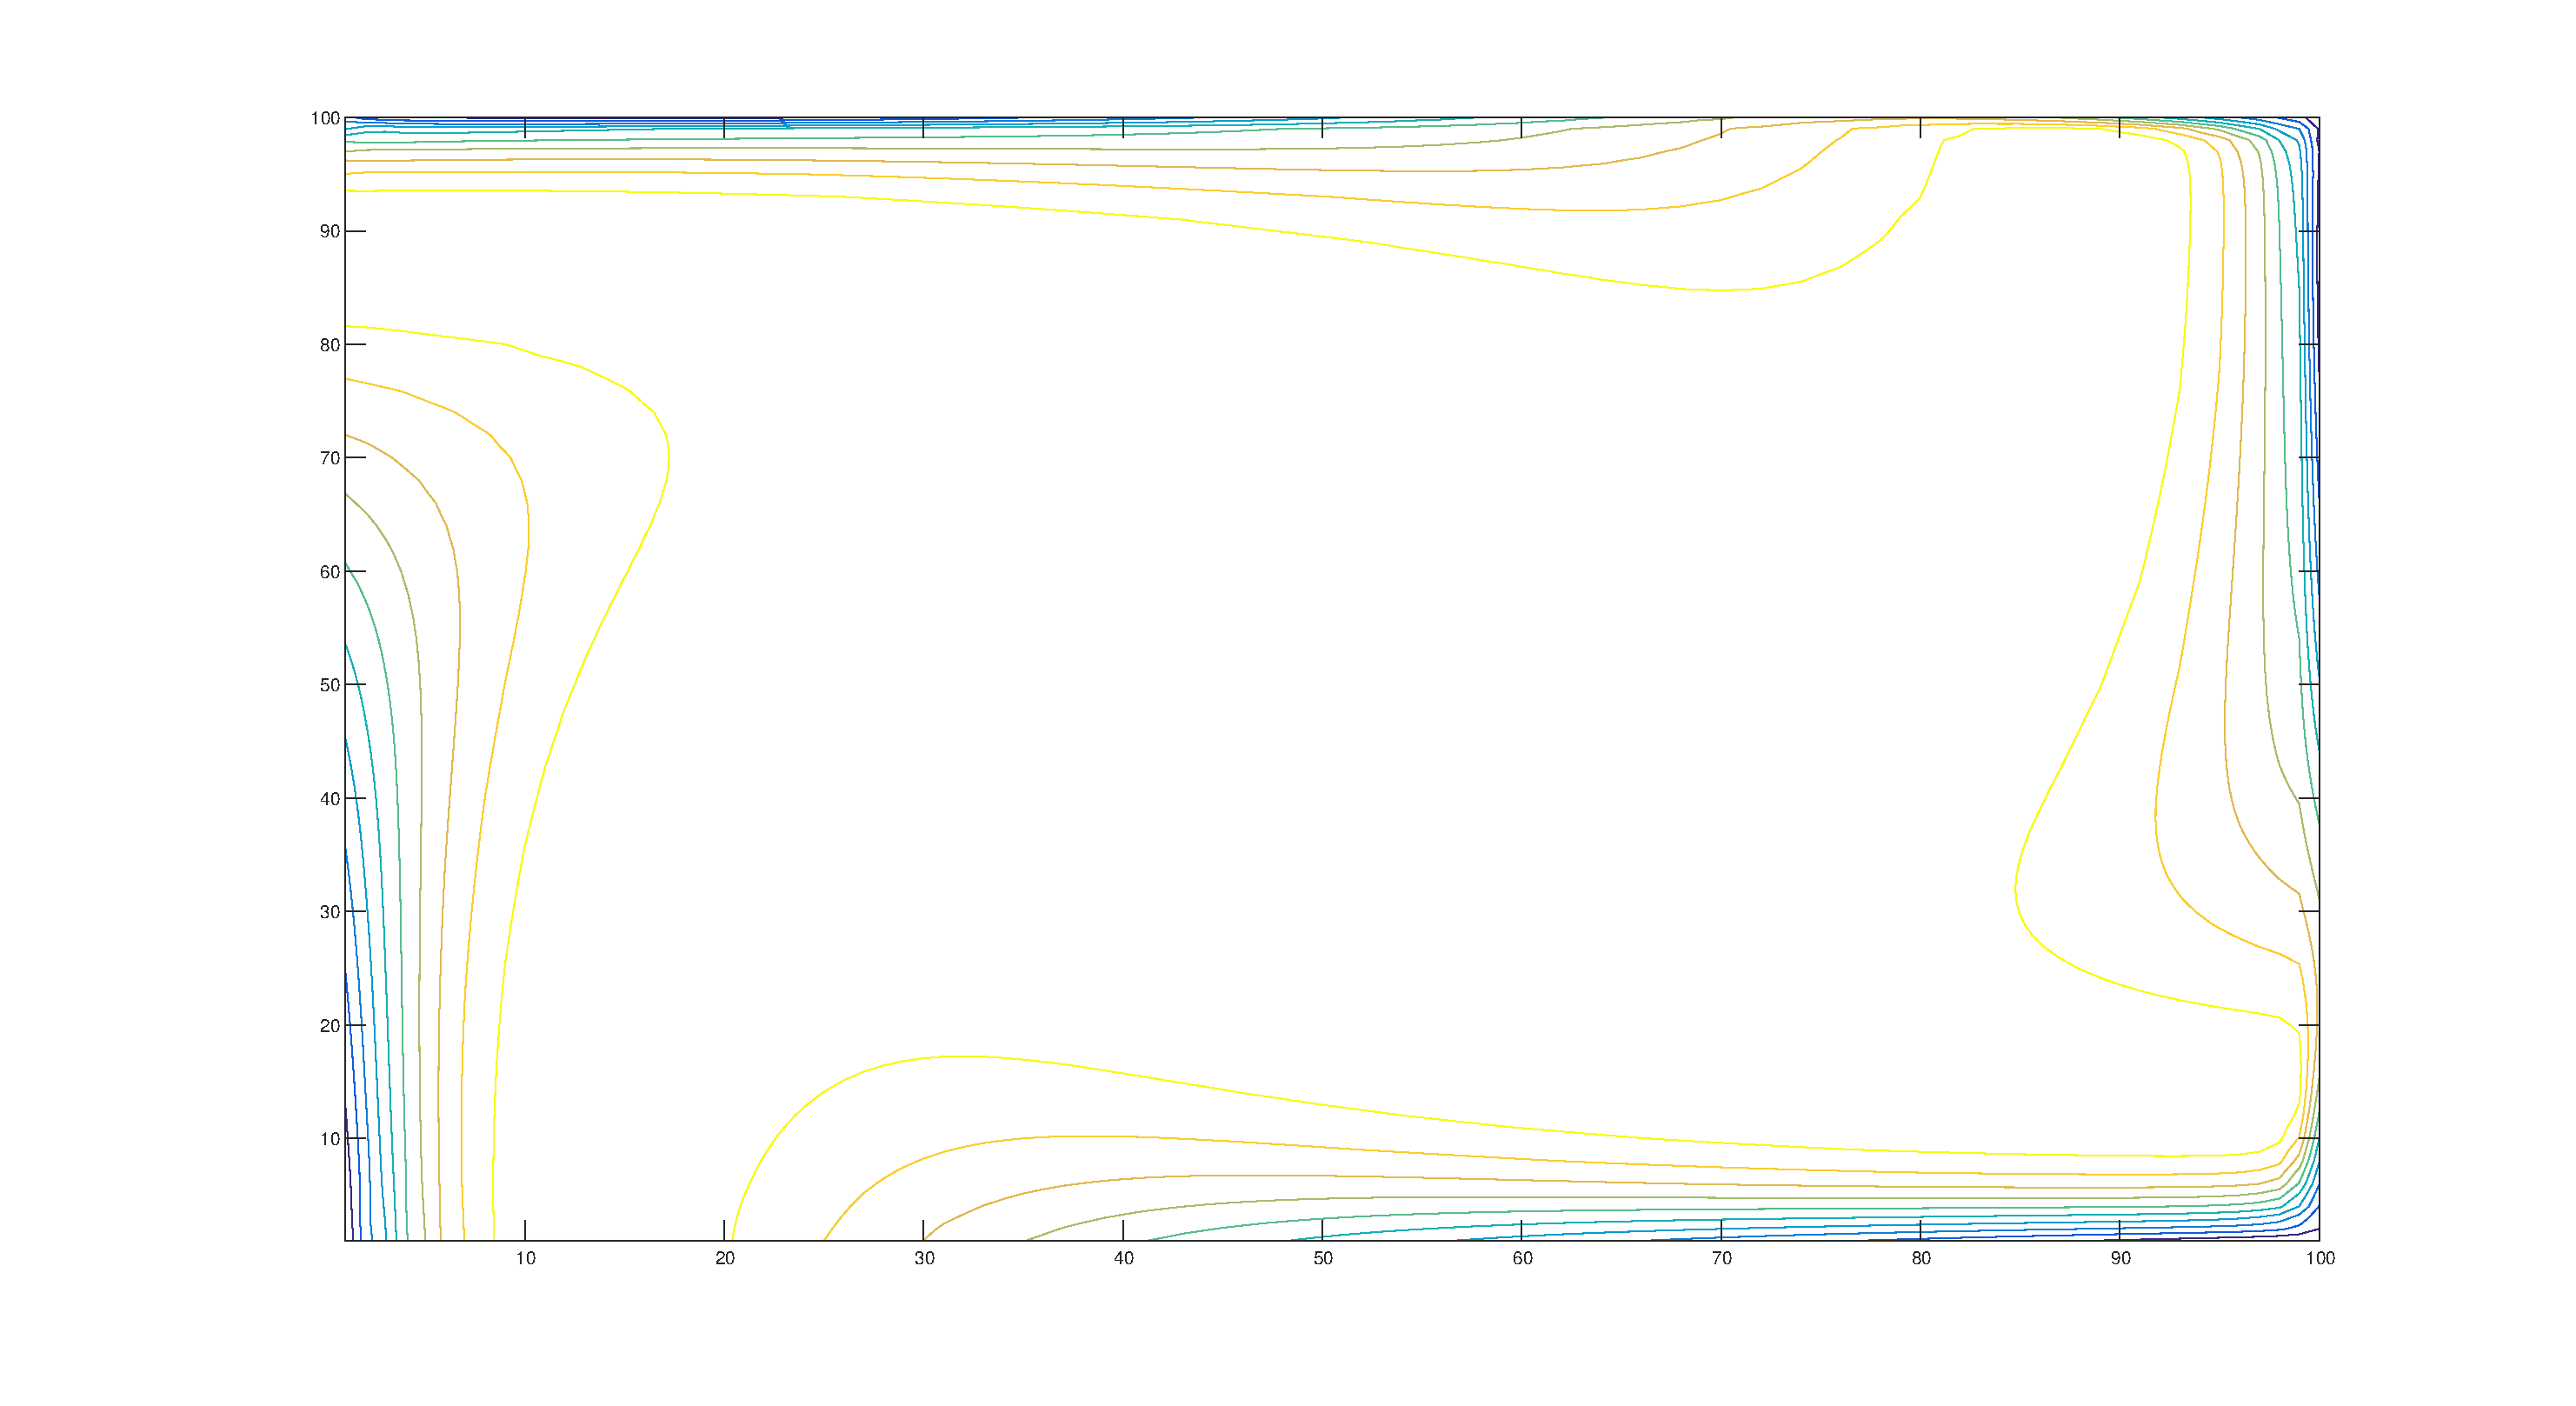
\includegraphics[width=0.45\textwidth,height=0.2\textheight]{./images/WENO3.eps}
}
\end{figure}
将$320\times 320$网格的解作为参考解,得到的2范数误差为
\begin{table}[H]
  \centering
  \begin{tabular}{cccc}
    $N$ & 40 & 80 & 160 \\
    \hline
    Upwind &0.1174&0.0525&0.0199 \\
    order& & 1.16 &1.40 \\
    WENO5 & 0.1171 &0.0524&0.0198 \\
    order& & 1.16&1.40 \\
  \end{tabular}
\end{table}
\subsection{结果分析}
迎风格式和WENO重构二者计算情况十分接近。迎风格式只具有一阶精度,但
WENO5的数值结果也只有一阶精度,这点比较奇怪。
\end{document}
